\section{Introduction}
During the requirements gathering process, four distinct components of the system were identified which form a pipeline of execution; \textit{Article Retrieval}, \textit{Keyword Extraction}, \textit{Graph Building} and \textit{Map Drawing}. Crucially, each is specified as being modular, allowing both for flexible extensibility and for alternative implementations to be tested directly against each other without requiring changes to the other components.

This chapter further decomposes these components to provide a detailed overview of the methodology used to implement them, followed by a discussion of the significant challenges and successes which arose during development.

\section{Code Reuse}
I developed the design of the system in Python 2.7 and JavaScript 1.7 using various open-source libraries and APIs for its ancillary functionality. The most notable are detailed below and discussed in context in the following sections.

\begin{itemize}[noitemsep]
	\item\textbf{FeedParser}\footnote{\url{http://pythonhosted.org/feedparser}}: A Python module for downloading and parsing RSS feeds.
	\item\textbf{Newspaper}\footnote{\url{http://newspaper.readthedocs.io}}: A Python library for downloading and extracting content and metadata from online articles.
	\item\textbf{lxml}\footnote{\url{http://lxml.de}}: A Python library for generating, parsing and manipulating XML and HTML.
	\item\textbf{NLTK (The Natural Language Toolkit)}\footnote{\url{http://www.nltk.org}}: A Python library for natural language processing and analysis.
	\item\textbf{Google Knowledge Graph Search}\footnote{\url{https://developers.google.com/knowledge-graph}}: The API for Google's knowledge base, which returns structured semantic search results.
	\item\textbf{D3.js}\footnote{\url{http://d3js.org}}: A JavaScript library for creating and manipulating interactive web visualisations and their underlying data.
\end{itemize}

\section{Article Retrieval}

The first stage of article retrieval is the parsing of RSS feeds, in order for article URLs and metadata to be extracted. The Python library FeedParser was used, as at the time of writing it provided the best support for RSS 0.9x, 1.0 and 2.0. The parsing process extracts a link, channel name, and the parsed publish date from every article in the feed, but it will also attempt to extract the author name if the \texttt{author} attribute is found.

Once the feed data has been extracted, it is used to construct an instance of \texttt{ArticleCollection}, which acts a wrapper around the contents of one or more feeds and provides the mechanism necessary to perform corpus-wide queries. The \texttt{Article} class encapsulates the functions for computing article-specific terms such as term-frequency for tf-idf, and the term-weighting component of tf-pdf. The result of this pre-processing stage is an \texttt{ArticleCollection} containing one or more serialisable \texttt{Article}s from one or more RSS feeds, where each \texttt{Article} contains extracted but unparsed data and associated metadata.

\section{Keyword Extraction}

The keyword extraction stage begins with the process of tokenising the body text of every article. Tokenisation here has three substages, all of which were implemented using NLTK (The Natural Language Toolkit for Python), and which are as follows:
\begin{enumerate}
	\item Sentence segmentation: Split the text into a list of sentences and remove sentence punctuation.
	\item Tokenisation: Split each sentence into a list of individual words and remove both whitespace and clause punctuation.
	\item Part-of-Speech (POS) tagging: Categorise each token according to its lexical class, e.g. adjective. This more of an extension to the tokenisation process than a part of it, but it is performed directly after tokenisation and is necessary for the next stage of processing.
\end{enumerate}
\begin{figure}[htbp!]
	\centering
	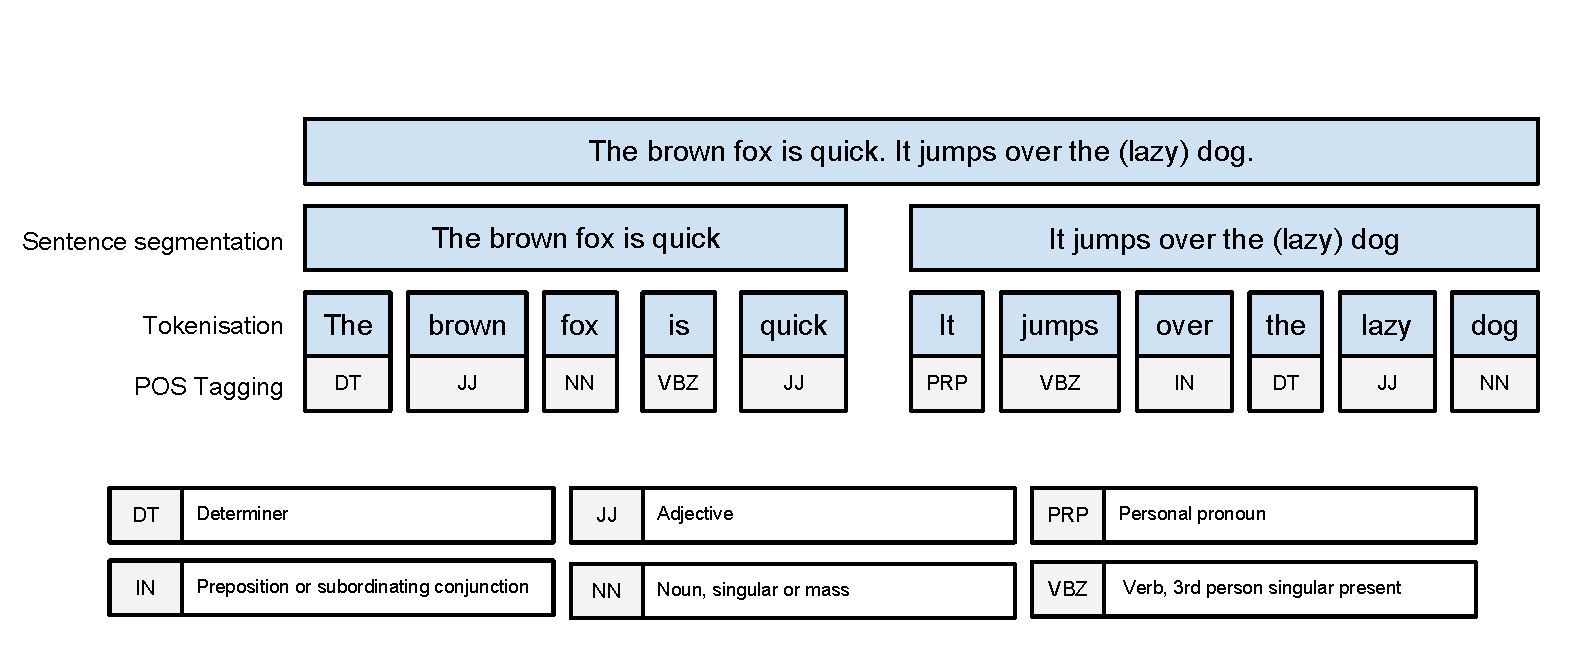
\includegraphics[width=\textwidth]{img/implementation/Tokenisation.pdf}
	\caption{Stepping through the tokenisation process}
	\label{fig:tokenisation}
\end{figure}

\subsection{Named Entity Recognition}

The second half of the keyword extraction process is exclusively concerned with named entities within articles. This is because, intuitively, the names of people, places, events companies and other \textit{things} form a set of strong candidate keywords. Restricting the candidates to entities alone reduces the search space by an order of magnitude when using frequency-based methods for keyword extraction, and bypasses the need for other natural language processing tasks such as stop-word removal and lemmatisation.

Once tokens have been POS tagged, named-entity chunking can be performed, again using NLTK. This process groups tokens into contiguous and non-overlapping \textit{chunks}, where each chunk is a named entity; typically a proper noun or some other noun phrase. It is possible for chunks to contain other chunks (consider the chunk `Bank of England', which contains the chunk `England'), but this is typically undesirable for entity recognition -- where we desire specificity -- so after chunking the tokens, we flatten the chunk structure so chunks cannot be any further decomposed.

At this stage, we have a list of chunks, each of which will be an eventual candidate for becoming a metro line. However, the chunks require some further processing before we can determine whether or not they are significant keywords.

\subsubsection{Substring Matching}
It is common stylistic practice in journalism to refer to the subjects of articles by their surnames. However, to avoid any confusion, the full names of those mentioned will often appear in the title or first few paragraphs of the article. If keyword strength is determined by frequency, then regardless of whether we use tf-idf or tf-pdf, we need every occurrence of an entity to refer to that entity by the same name; preferably the most specific, which is typically the longest.

During this stage of disambiguation, we only consider entities with more than one mention in the source text as candidates. This is because the chunking process can produce false positives by combining unrelated adjectives with valid chunks, but the likelihood of the same false positive being produced twice or more in the same article is low.

Let $P$ denote the set of entities with more than one occurrence in the source article; $S$:
\begin{align*}
P &= \{e\;|\;\text{occurences}(e, S) > 1\}.
\intertext{$\forall (e_1, e_2) \in \{P\times{P}\;|\;$length$(e_1)\;<\;$length$(e_2)\}, $ if $e_1 $ is a substring of $e_2$, we call $e_1$ an \textit{alias} of $e_2$. Let $A$ be the set of alias pairs in $S$;} 
A &= \{(a, e) \;|\;a \text{ is an alias of } e\}
\intertext{We require the first term of every pair in $A$ to be unique, but there is no such constraint for the second term ($e$); this allows multiple aliases to map to the same entity. For example,} 
 & \{(\text{`Zuckerberg'}, \text{`Mark Zuckerberg'}), (\text{`Zuck'}, \text{`Mark Zuckerberg'})\} 
%\intertext{and}
%& \{(\text{`Zuck'}, \text{`Zuckerberg'}), (\text{`Zuckerberg'}, \text{`Mark Zuckerberg'})\}
\intertext{would be unambiguous and therefore valid, but}
 & \{(\text{`Mark'}, \text{`Mark Zuckerberg'}), (\text{`Mark'}, \text{`Zuckerberg'})\}
\intertext{would not be. Let $U$ be the set of unambiguous alias-entity pairs in $S$:}
U &= \{(a, e) \;|\; (a, e)\in{A} \cap \forall(e_1, e_2)\in A, \; a = e_1 \implies e = e_2 \}
\end{align*}

We have a reasonable degree of confidence that for every alias-entity pair $(a, e) \in U$, occurrences of $a$ in the source text can be replaced by $e$, making $e$ a stronger candidate for keyword detection. Pairs in $(a, e) \in A\setminus{U}$, that is, aliases which could map to multiple entities in the source, are disregarded at this stage and left unchanged.  Algorithm \ref{alg:u} illustrates how, given a list of entities, we can find the unambiguous pairs deterministically. 

\begin{algorithm}
\label{alg:u}
 \caption{Finding unambiguous alias-entity pairs}
 \KwData{$names$: a list of recognised entities}
 \KwResult{$U$: the set of unambiguous pairs in $names$}
 $U \gets$ \{\}\;
 \ForEach{$e_1, e_2$ $\in ($names $\times$ names$)$}{
   \If{len($e_1$) $>$ len($e_2$)}{
   	swap($e_1$, $e_2$) \;
   }
  \If(\tcc*[f]{If $e_1$ is a substring of $e_2$}){$e_1 \in e_2$}{
   	\eIf{$e_1 \notin U$}{
   	  $U$[$e_1$] $\gets e_2$ \tcc*[r]{$(e_1, e_2)$ are a candidate pair}
    }{
      delete $U$[$e_1$] \tcc*[r]{$e_1$ is now ambiguous, so remove it}
    }
   }
 }
\end{algorithm}


\subsubsection{Entity Disambiguation with Knowledge Graph}

The process described above is a simplistic approach which only addresses the matching of partial to full name mentions. In comparison, entity disambiguation describes the process of determining the identity of entities in a body of text. Performing this process on the sentence `The UK has voted to leave the EU,' should identify `UK' as 'The United Kingdom' and `EU' as 'The European Union'. As advanced methods for entity disambiguation are both complex and computationally expensive, I did not attempt to implement a formal method for this. 

Instead, the list of recognised entities are queried against Google's publicly accessible Knowledge Graph API, which returns a list of potential results as Schema.org\footnote{http://schema.org is an online hierarchy of types managed by W3C (The World Wide Web Consortium)} types. Knowledge Graph is the service which replaced Freebase in 2015, and currently contains over 70 billion facts \citep{knowledgegraph}.

\cite{EntityDisambiguationForKnowledgeBasePopulation} identify three key challenges in entity linking using knowledge bases; name variations, ambiguity, and absence. Absence describes the lack of a corresponding entry for the entity in the knowledge base, which is not an easily tackled problem. Ambiguity is a consequence of the polysemy of many names and acronyms and requires disambiguation to be performed using more contextual methods. 

Both of these problems are left unsolved in the design and implementation of the system due to scoping constraints. However, naïve substring matching combined with the use of Knowledge Graph and some empirical parametric estimation are enough to disambiguate name variations of all forms (partial matches, abbreviations, and acronyms) to a sufficient degree, and with surprising accuracy.

The key to using Knowledge Graph for disambiguation lies in its most vaguely defined return value. Each result has a score attributed to it by Knowledge Graph, which is an indicator the strength of the match between the entity and the original query. Results are sorted by descending score; the higher the \texttt{resultScore}, the better the match. Although there is no defined upper limit for this value and no official documentation on how the score is derived, comparing the scores of the top two results for a query can provide a measure of certainty, for all but particularly esoteric or unknown entities.

We specify a threshold $\frac{1}{t}$, which is roughly proportional to the likelihood of accepting a false positive match. Then, if dividing the score of the first result by the score of the second yields a number greater than $\frac{1}{t}$, we accept the match. Provisionally we set $t=0.5$; a discussion of how I arrived at this value is provided in the next section.

Using a knowledge base for disambiguation also inadvertently solves another problem I encountered while parsing articles, this time as a result the expositional style of journalistic writing. While keywords are typically nouns or noun phrases, they can also appear in the form of denominal adjectives. These adjectives are derived from nouns; e.g. `French' implies `France' might be a keyword. Denominal adjectives are not amenable to traditional stemming or lemmatising, but querying Knowledge Graph for `French' returns a top match of `France' with a \texttt{resultScore} of 432.42807; more than four times larger than the next result.

Given a list of entities $E$, and top two results of a Knowledge Graph query for each $e \in E$; $R_e(1)$ and $R_e(2)$ with scores $S_e(1)$ and $S_e(2)$ respectively, our aim is to return a set of pairs mapping zero or more entities in $E$ to their disambiguated forms;

\begin{align*}
K &= \bigg\{(e, R_e(1))\;|\;\frac{S_e(1)}{S_e(2)} > \frac{1}{t}\bigg\}
\end{align*}

Algorithm \ref{alg:kg} describes this process. For higher values of $t$, the likelihood of accepting a false positive increases, and for lower values, the likelihood of accepting a false negative increases. For corpora which do not contain references to public figures and place names, choice of $t$ should be empirically tuned against the prevalence of the expected entities.

\begin{algorithm}
\label{alg:kg}
 \caption{Entity disambiguation with Knowledge Graph}
 \KwData{$names$: a list of recognised entities \\ 
 		\hspace{1.2cm}$t$: the acceptance threshold for results, default = 0.5}
 \KwResult{$K$: a set of disambiguation mappings for elements in $names$}
 $K \gets$ \{\}\;
 $T \gets 1\div{t}$\;
 \ForEach{$e \in names$}{
 	$results \gets$ KnowledgeGraphResults($e$)\;
 	\If{len($results$) $>$ 1}{
	   \If{$results$[0].score $\div$ $results$[1].score $> T$}{
	   		$K[e] = results[0].name$\;
	   }
	}
 }
\end{algorithm}

It is unclear what should become of queries that Knowledge Graph only returns a single result for, but in this implementation they are ignored.

\subsubsection{Determining Optimal Values for $t$}

Empirically, I found the best values for $t$ are in the range $0.35 < t < 0.65$, meaning we accept top results which are at least 1.5x-3x higher than the next best candidate. To determine this, I logged all the disambiguation pairs found in 20 articles from the BBC Politics RSS feed, letting $t$ range over \{0.3, 0.5, 0.7, 0.9\}. I then manually classified the pairs as either true or false positives, where a true positive indicates a correctly identified entity, and a false positive is either an incorrectly identified entity or a non-entity which was not identified at all. Figure \ref{fig:dthreshold} shows the results of this investigation.

\begin{figure}[htbp!]
	\centering
	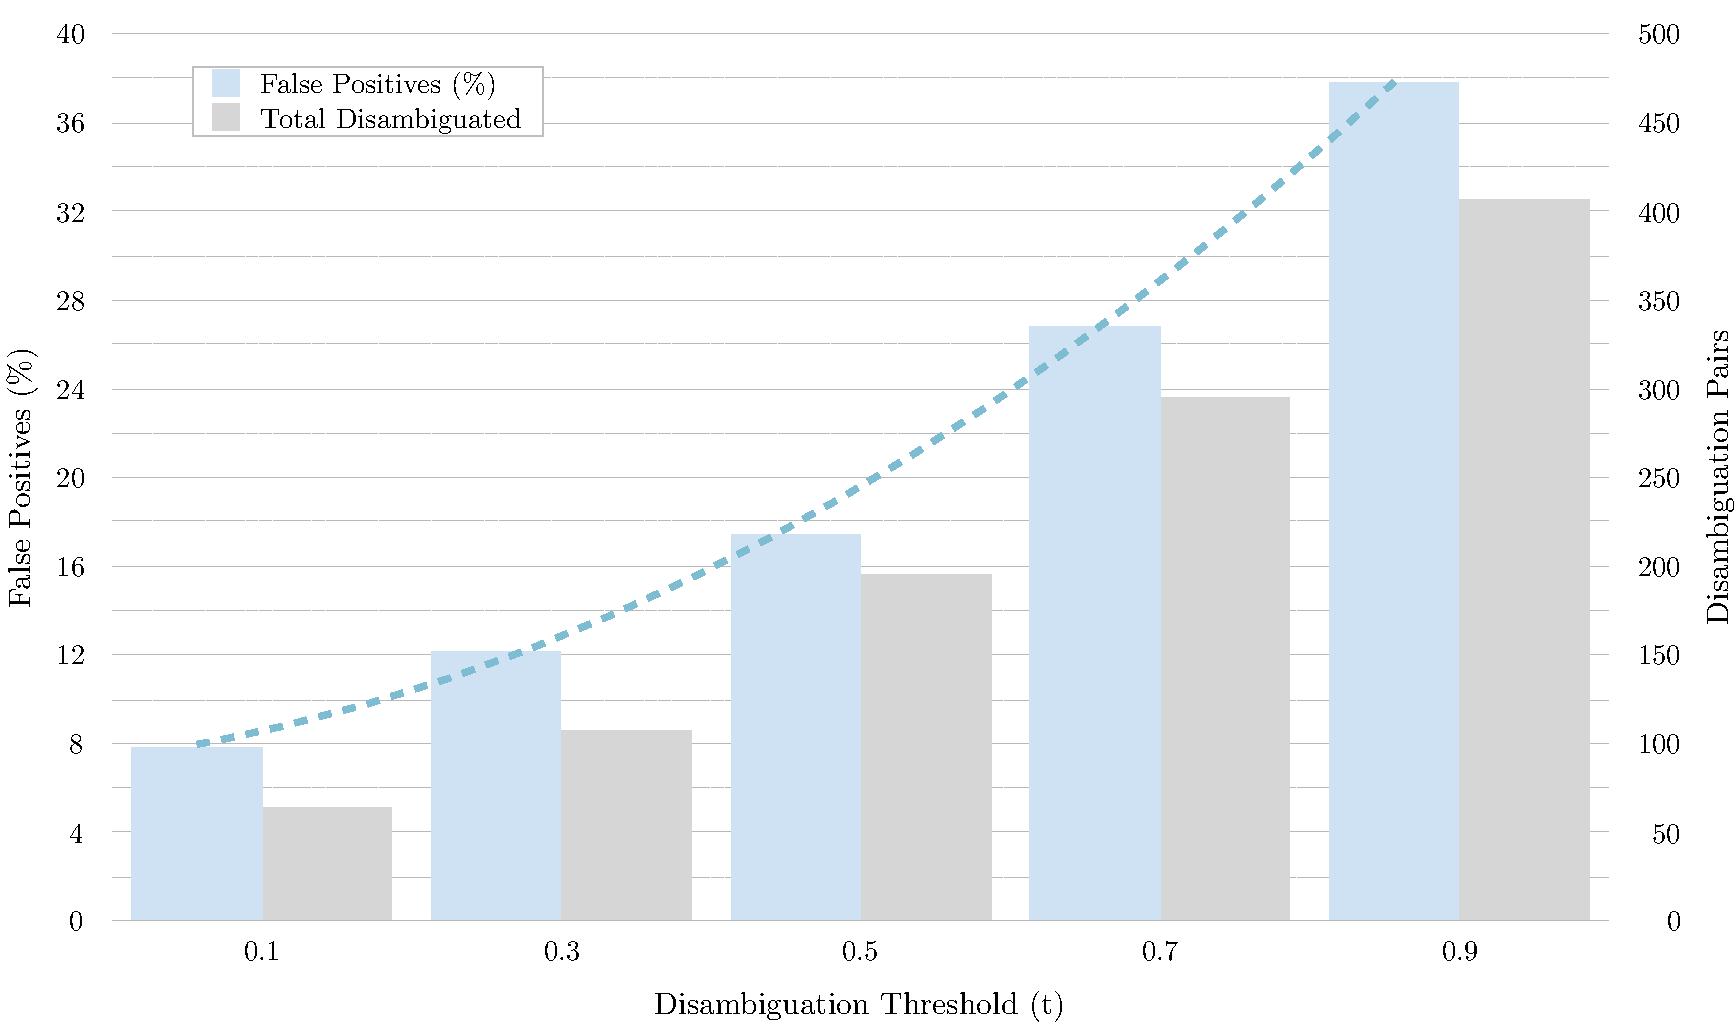
\includegraphics[width=\textwidth]{img/implementation/DisambiguationThreshold.pdf}
	\caption{Disambiguation threshold against pairs found and false positives (\%)}
	\label{fig:dthreshold}
\end{figure}

Although we see a reduction in false positives for smaller values of $t$, the trend-line illustrates that this is a game of diminishing returns; reducing $t$ from 0.3 to 0.1 only reduces the false positives by 4.34\%, but it leads to 43 fewer pairs being identified\footnote{Since it is both extensive and tangential to the focus of the project, raw data for this table can be found at \url{http://bit.ly/DisambiguationThresholding}.}. 

There is a clear trade-off between the accuracy of the disambiguation and the number of false negatives we discard, but the cost of false positives in this case is less than the cost of false negatives. While a false positive could result in unrelated entities appearing as keywords for certain articles, the likelihood of the same false positive appearing with high frequency in enough articles to result in an erroneous metro line is incredibly low. In contrast, the cost of disregarding a false negative could result in articles being left off certain metro lines altogether. It is for this reason that we don't simply choose the value of $t$ which yields the minimum ratio of false positives.

\subsection{Choosing a Term-Weighting Metric for Keyword Ranking}

Given a set of disambiguated entities for every article, the union of which forms a set of candidates keywords or \textit{metro lines} for the collection, we must now determine which keywords are the most relevant. To do this, the two term-weighting methods described in Chapter \ref{c:litreview} will be revisited; tf-idf \citep{tfidf} and tf-pdf \citep{TopicExtractionfromnewsArchiveUsingTFPDFAlgorithm}. Both were implemented in the system so they could be compared directly against each another.

From an implementation perspective, the main difference between these two algorithms are the level at which they operate. tf-idf ranks keywords on a per-article basis, returning a vector of an article's keywords and their corresponding score against the background corpus. In contrast, tf-pdf is specified at corpus level and only returns a single metric for a given word; the sum of its significance across the whole corpus. In tf-pdf, corpuses have one or more \textit{channels}, which contain articles. In our case, channels can be conveniently defined as RSS feeds from different publishers. 

\citeauthor{TopicExtractionfromnewsArchiveUsingTFPDFAlgorithm} argue that tf-pdf is a more suitable metric for news corpora, because it discriminates between articles which originated from the same channel and articles in different channels, allowing keywords which are highly (and uniformly) frequent in one channel to be identified as significant in documents from a different channel. Similarly to tf-idf however, this process can be used to produce a vector of pairs of an article's highest ranked keywords. The actual scores attributed to keywords by either algorithm are not of direct importance, since it is only relative scores we use to construct the keyword vectors.

%\subsubsection{Implementation of tf-pdf Vectorisation}
%
%\begin{itemize}[noitemsep]
%	\item $D$ = The number of channels in the corpus;
%	\item $K_c$ = The total number of terms in channel $c$;
%	\item $F_{tc}$ = Frequency of term $t$ in channel $c$;
%	\item $n_{tc}$ = The number of articles in channel $c$ where term $t$ occurs;
%	\item $N_c$ = The total number of articles in channel $c$.
%\end{itemize}
%\begin{equation}
%	\text{tf-pdf}(t) = \sum_{c=1}^{c=D}\frac{F_{tc}}{\sqrt{\;\sum\limits_{k=1}^{k={K_c}}{F_{kc}}^2}}\times\text{exp}{\bigg(\frac{n_{tc}}{Nc}\bigg)}
%\tag{\ref{eqn:tfpdf}}
%\end{equation}

Regardless of which algorithm is used, the advantage to restricting the set of candidates to named entities becomes quickly apparent. Figure \ref{fig:tokensentities} shows the number of tokens against the percentage of extracted entities for 40 articles from the BBC's Politics RSS Feed.\footnote{http://feeds.bbci.co.uk/news/politics/rss.xml (Accessed: 27/02/2017, Full data in Appendix \ref{tab:entitiestokens})} The interquartile range shows 50\% of articles had entities comprising 5.4\%-8.2\% of their tokens after stop-word removal. With the mean equal to 6.65\%, the implications of this are a search space which can be reduced by a factor of more than ten. Although performance optimisation was not specified in the aims of the project, gains of this nature are still significant.

\begin{figure}[htbp!]
	\centering
	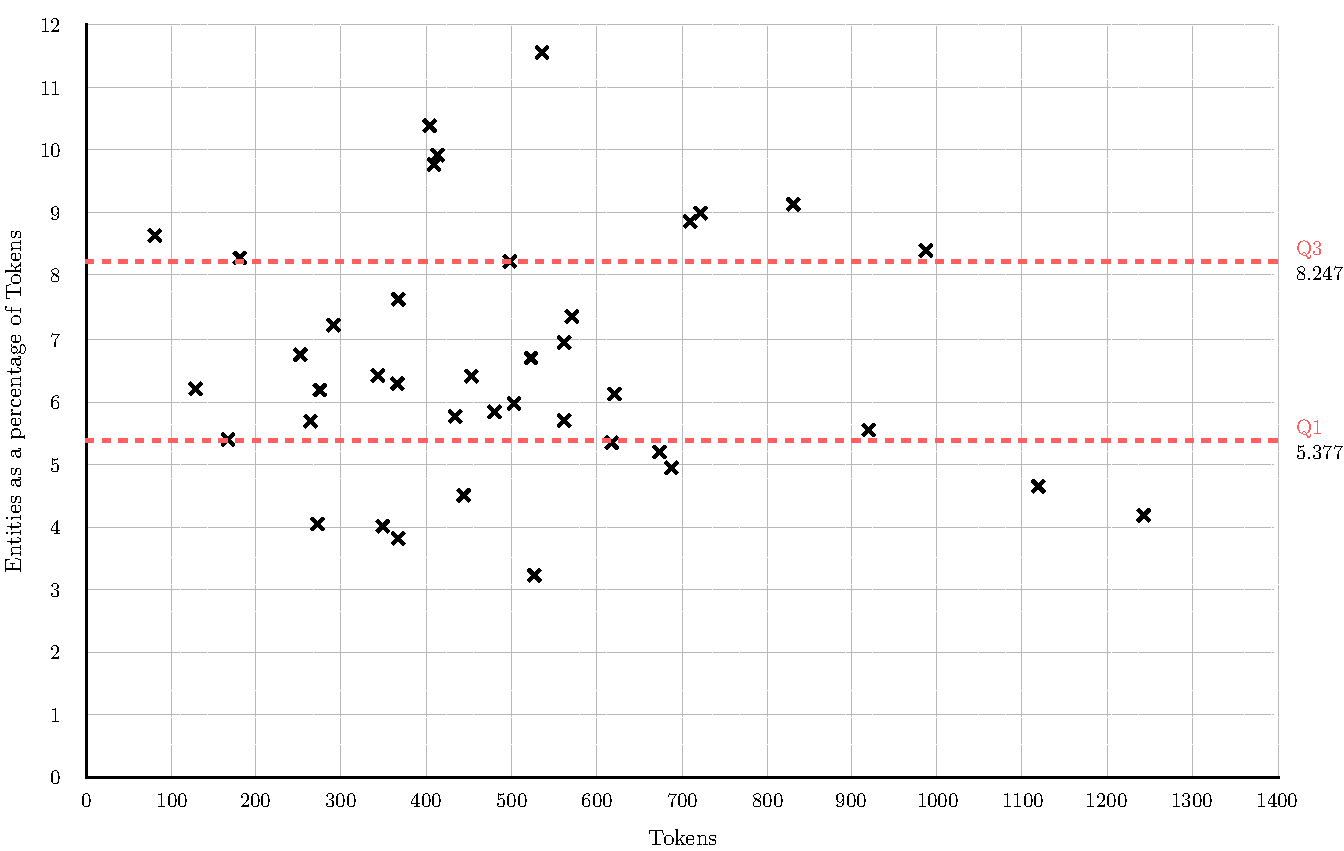
\includegraphics[width=\textwidth]{img/implementation/TokensEntities.pdf}
	\caption{Entities as a percentage of Tokens across 40 BBC Politics articles.}
	\label{fig:tokensentities}
\end{figure}

At this point, given optional user-specified lists of keywords to either \textit{include} or \textit{ignore}, we can filter out or boost the scores of articles which mention these topics, which in the case of \textit{include} will guarantee the keyword is selected as a metro line in the map, as long as it is mentioned in at least two articles. 

The function of the \textit{ignore} set is not to blacklist certain topics, as it will have no effect on articles which contain ignored keywords being placed on other metro lines. Instead, it performs domain specific stop-word removal for metro line candidates, preventing non-useful keywords with inevitably high scores (such as `United Kingdom' for a metro map based on a UK news corpus) from being selected. During implementation, it was found to be useful to automatically append the names of every news publisher (e.g. `The Guardian') in the feeds to the \textit{ignore} set, as well as the names of the feeds themselves. This forces the system to select more specific candidates, even though their scores may be significantly lower.

While implementing the \textit{ignore} functionality that the differing results of using tf-idf and tf-pdf on the same corpus became obvious. Because tf-idf penalises words which appear with low but constant frequency across a number of documents, keywords we intuitively would wish to ignore such as `United Kingdom' are not scored as highly as they would be with tf-pdf. This is in line with the findings of \citeauthor{TopicExtractionfromnewsArchiveUsingTFPDFAlgorithm}; tf-pdf does do a better job at detecting low-frequency keywords which are consistent across many documents. However, this behaviour is exactly the opposite of what we desire from our metro lines; those low-frequency keywords are most likely already known or could be easily inferred by a user reading the map. Therefore, it is my recommendation that tf-idf be given preference in any implementations of this or similar systems, where the names of more specific low-level themes are being sought.

\clearpage

\section{Graph Building}

The key challenge in graph building is generalising the characteristics of a good overview, from both news consumer and metro map user perspectives. It is at this point that a significant difference between this system and the work of \cite{MetroMapsOfScience, GeneratingInformationMaps, InformationCartographyPre} becomes apparent. 

\citeauthor{GeneratingInformationMaps} generated maps in response to a query (such as the name of an event or time) period, meaning the entire map would then be oriented around that query. In contrast, in our system the only query is an implied one; ``What's going on today?" which offers no starting point for choosing metro lines. Instead of a query-based search problem, we have a multi-document summarisation problem. While they were choosing a set of lines to fit a given query, we are concerned with choosing a set of lines which best cover an entire corpus.

\subsection{Extending the Definition of Coverage to Paths}

Our starting point is a corpus of articles and their associated keyword vectors, which form a metro map by \citeauthor{GeneratingInformationMaps}'s definition, but one with too many edges and paths (metro lines) to be readable in practice. Therefore, in order to intelligently prune the number of paths to some fixed upper bound, we need a metric for comparing the relative importance of paths within a corpus.

To do this, we first recall the original definition of document coverage (equation \ref{eqn:doc-coverage} \citep{GeneratingInformationMaps, MetroMapsOfScience, InformationCartographyPre}), where $d$ is a document, $w$ is a keyword, and $\mathcal{W}$ is some normalised measure of term-frequency, such as tf-idf.

\begin{equation}
	cover_{d}(w) : \mathcal{W} \rightarrow [0,1]
	\tag{\ref{eqn:doc-coverage}}
\end{equation}

In order to compare candidate metro lines, we build on this definition of coverage to extend it to paths (Equation \ref{eqn:line-coverage}).

\begin{equation}
	Coverage(\mathcal{P}) = {|\mathcal{P}|}\sum_{d\,\in\,\mathcal{P}}\frac{cover_{d}(\mathcal{P})}{|\{\,p\in{\Pi}\;|\;d \in p,\,p \neq \mathcal{P}\}|}
	\label{eqn:line-coverage}
\end{equation}

Here, the extent to which a path $\mathcal{P}$ covers a document $d$ within a corpus $\mathcal{D}$ is proportional to its tf-idf coverage of that document and inversely proportional to the number of other candidate paths which \textit{also} cover that document. The coverage of the entire corpus by $\mathcal{P}$ is then given the sum of its coverage of the articles along it multiplied by the length of the path, with high coverage being desirable.

It is important to note that although with the final multiplication we show preference to longer metro lines, the objective of the system is not simply to maximise the number of articles which are included on the generated maps. This could easily be achieved by choosing the most nonspecific universal keywords as metro lines, but the resulting map would be uninformative and would most likely do nothing to counter news overload. It is in the nature of summarisation that not all information can be preserved, and in doing this kind of graph selection, the information lost is those articles which don't form links to the significant topics within the corpus.

%This means tf-idf is preferable to tf-pdf, because while tf-idf is really good at identifying high-level topics which cover a lot of articles, it can cover those articles very poorly and generate a) too few lines, which; b) all run adjacent to each other anyway (see the next section).

\subsection{Penalising Affinity}

The principle of topic connectivity was the basis for choosing the metro map visualisation. Without it, we have simply generated a set of two-dimensional timelines with no contextual links. However, maps which are overly connected will quickly become unusable. In particular, maps where multiple lines runs adjacently through more than two nodes (see figure \ref{fig:lowaffinity}) a sign of poor line choice. This is not simply hyper-connectivity, but correlation between two or more lines, often resulting from keywords which are semantically close.

\begin{figure}[htbp!]
	\centering
	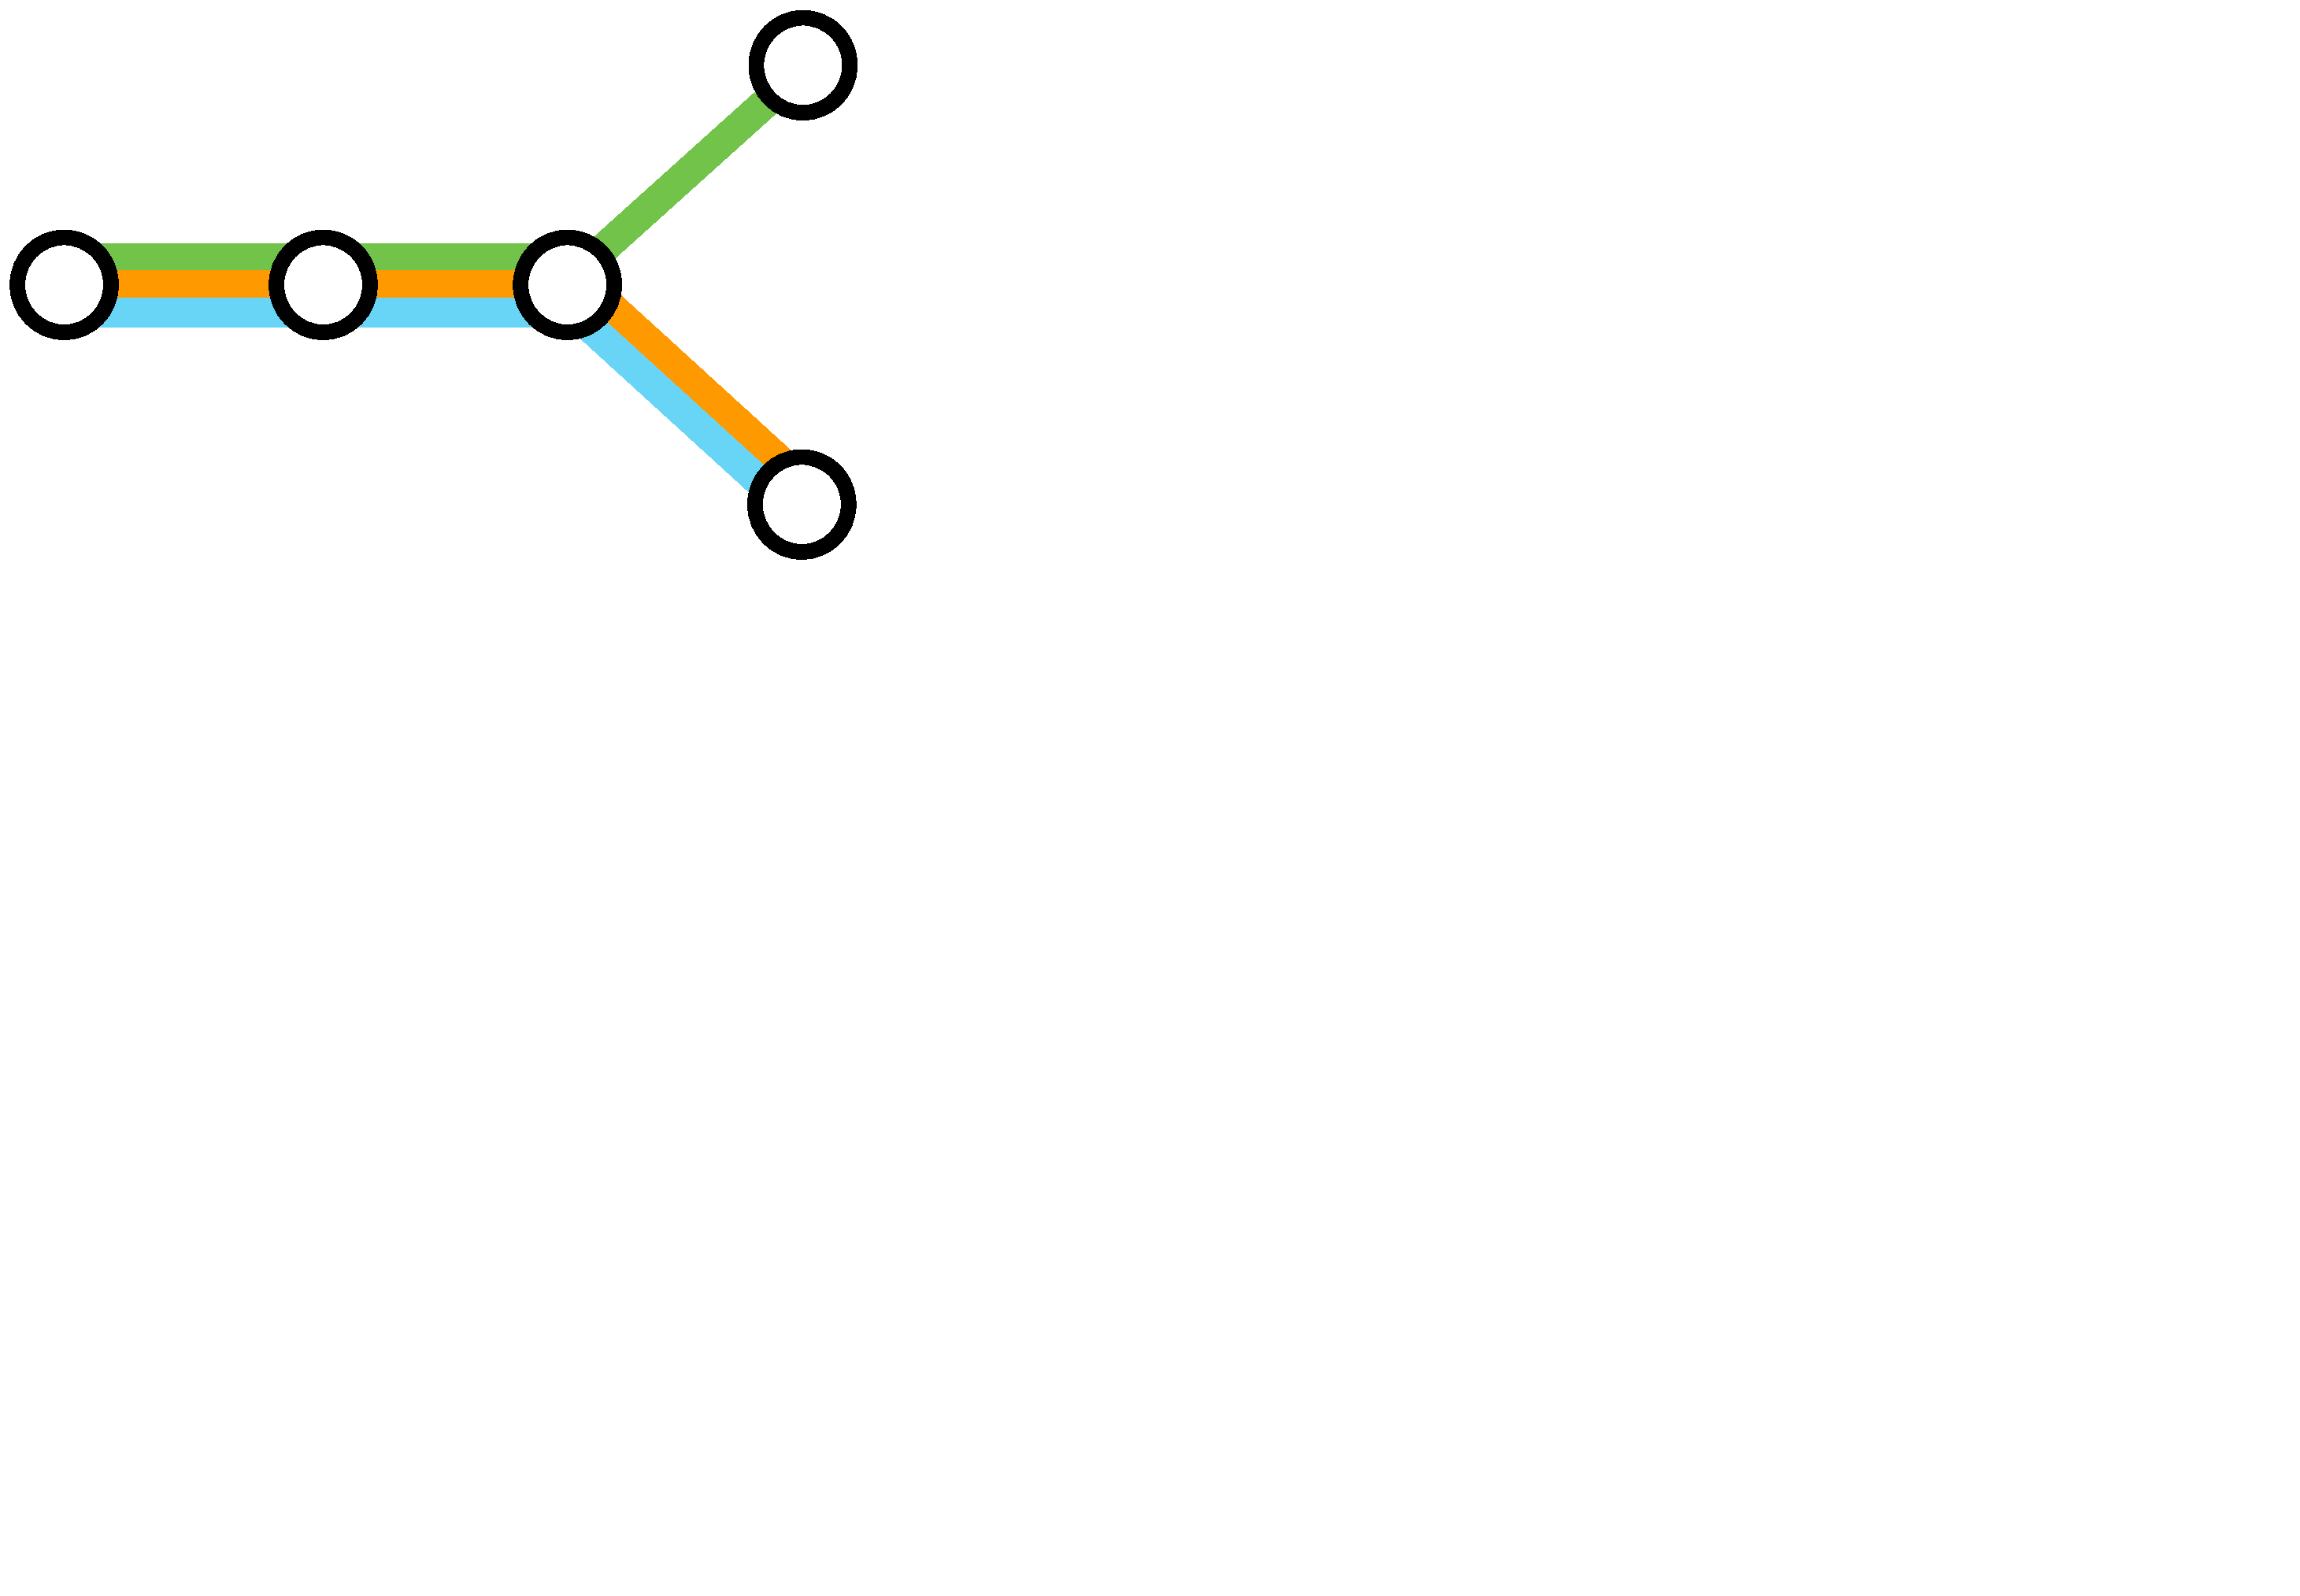
\includegraphics[width=.5\textwidth]{img/implementation/lowaffinity.pdf}
	\caption{An example of three metro lines, each with high affinity.}
	\label{fig:lowaffinity}
\end{figure}

We call this function of two lines their \textit{affinity}, and define the affinity of a single line as the sum of its affinities over the set of paths, excluding itself.

\begin{equation}
	Affinity(\mathcal{P}) = \frac{1}{|\mathcal{P}|} \sum_{p\,\in{\,\Pi}} 2^{|\{\,d\,|\,d\,\in\,{\mathcal{P}}\,\cap\,d\,\in\,{p},\,p\,\neq\,\mathcal{P}\}|}
\end{equation}

The affinity of two lines is defined as the number of articles they have in common, raised as a power of two. The effect of the power is illustrated in Figure \ref{fig:abcaffinity}. On the right, line $a$ (orange) which shares one article with line $b$ (green) and another with line $c$ (blue) does not indicate as strong a correlation as on the left, where $a$ shares two articles with $b$ and none with $c$. As with line coverage, we penalise shorter lines.

\begin{figure}[htbp!]
	\centering
	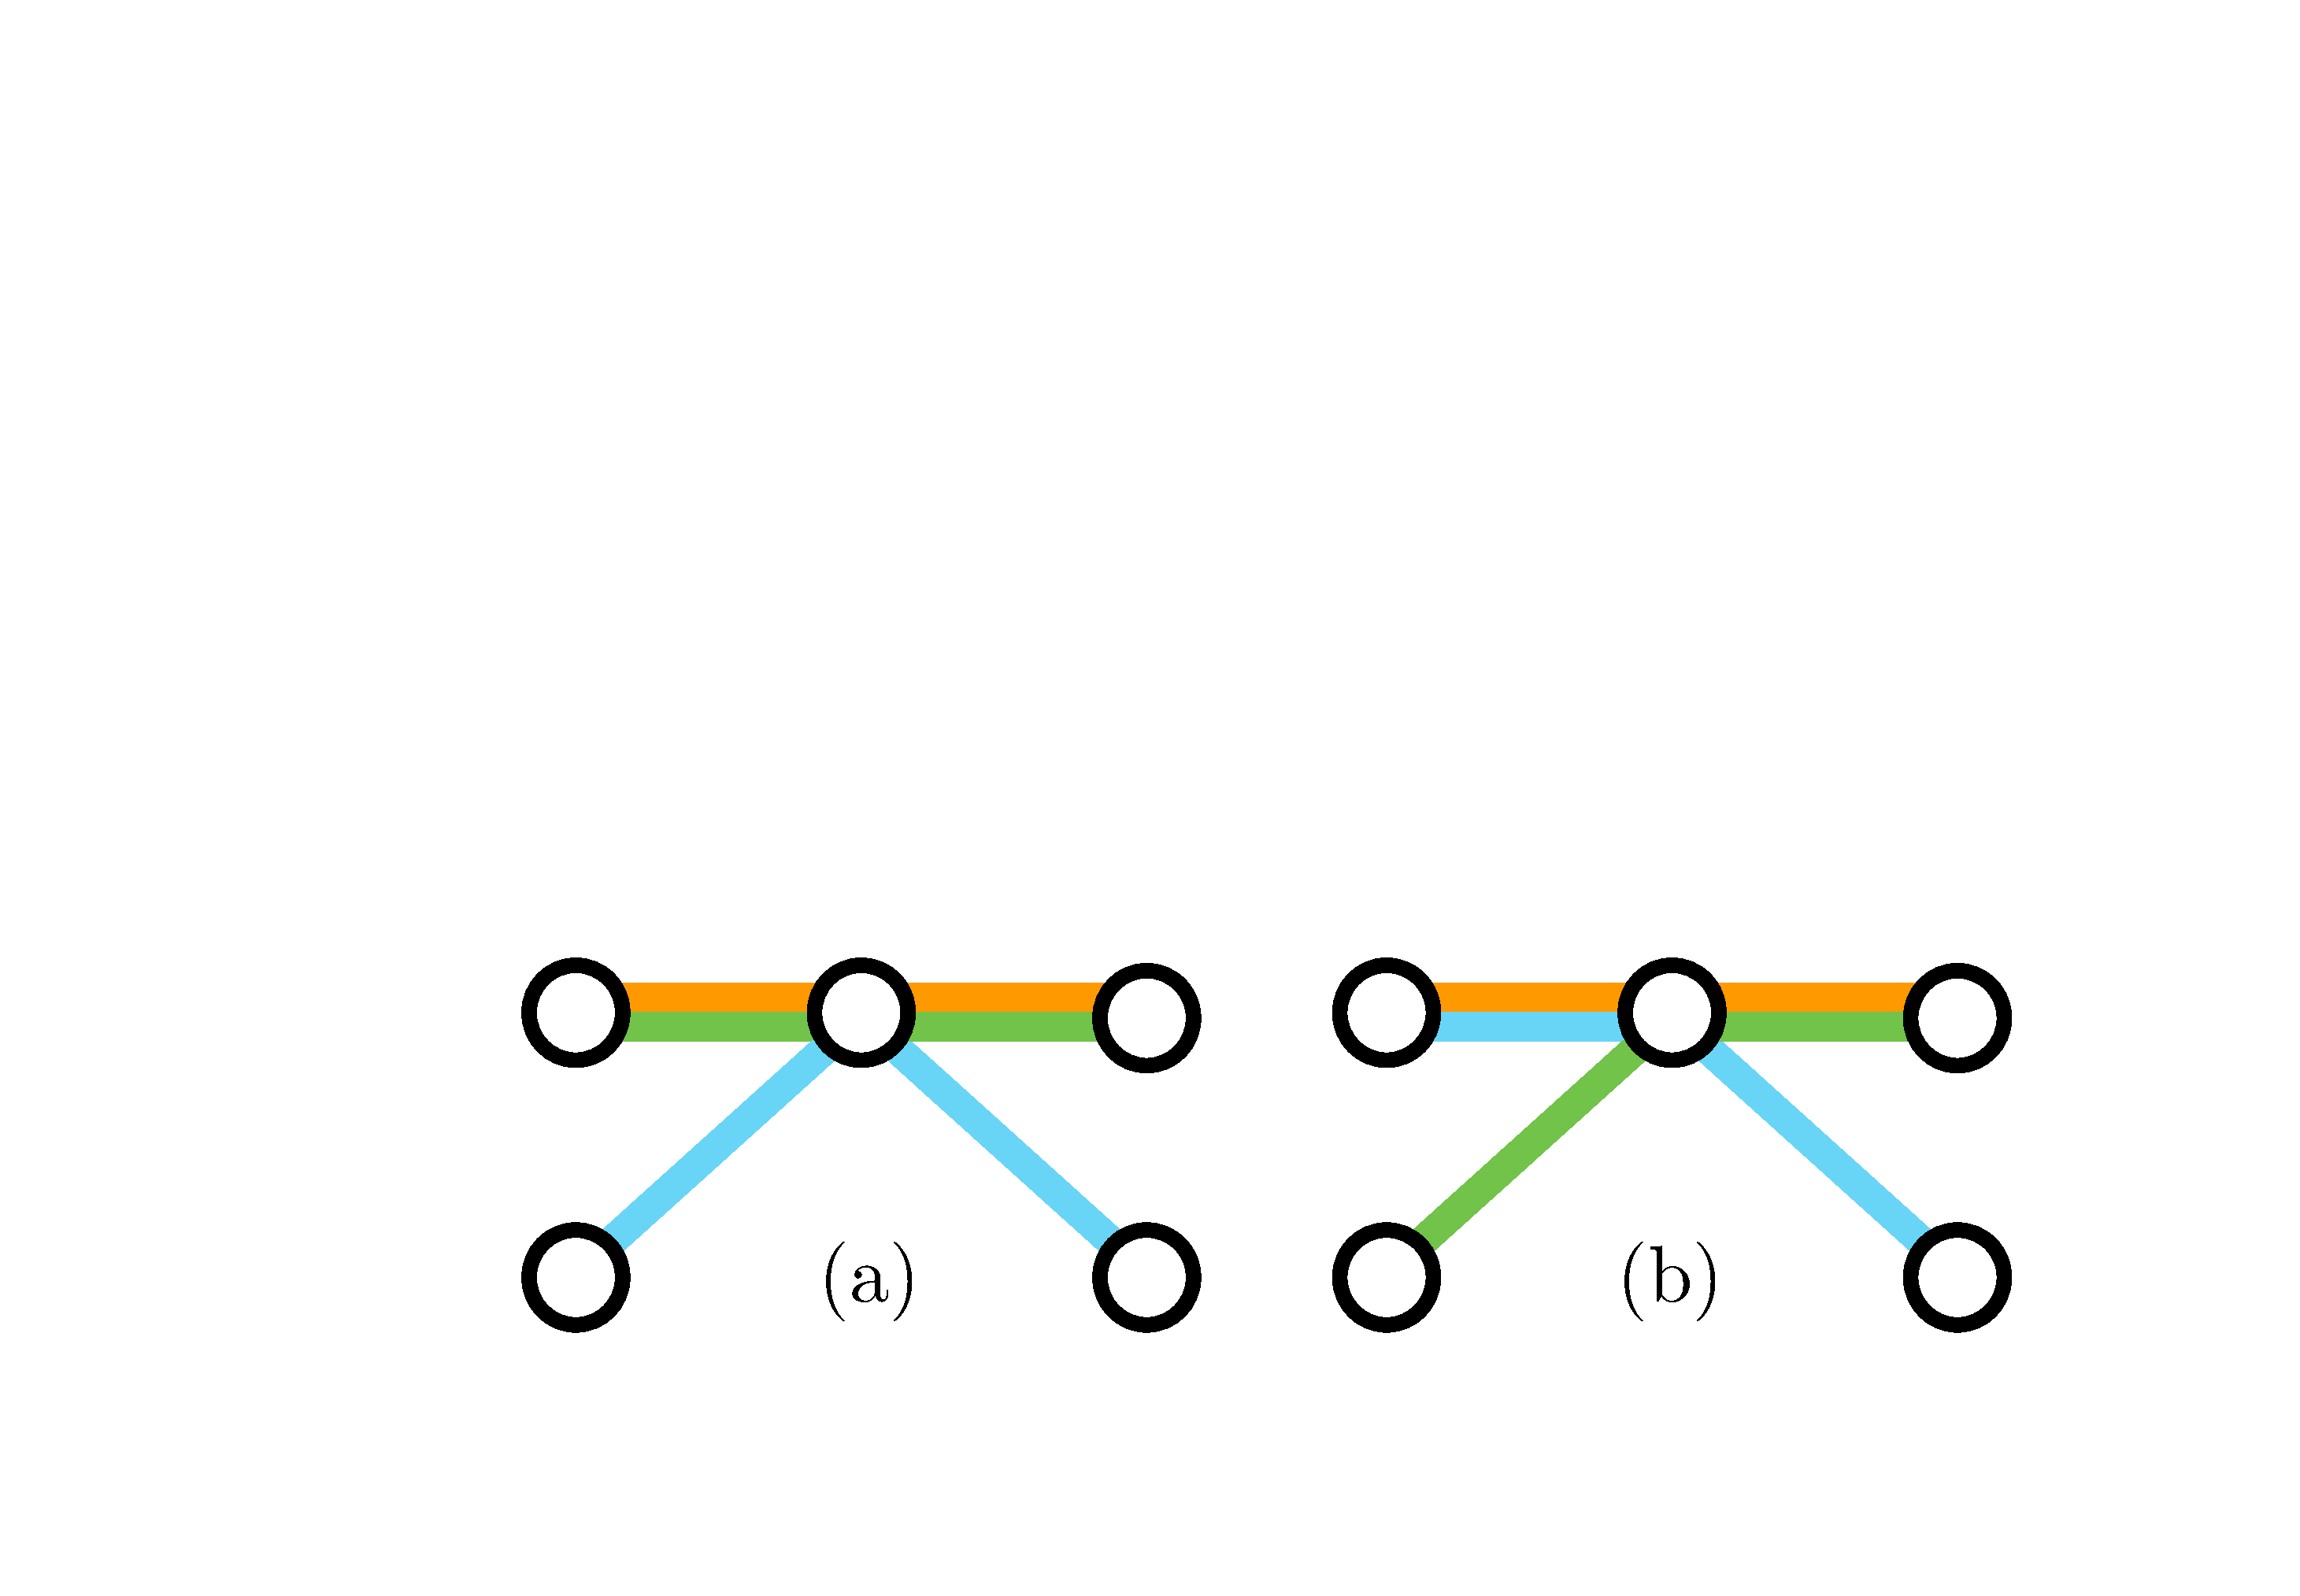
\includegraphics[width=\textwidth]{img/implementation/abcaffinity.pdf}
	\caption{`Run-on' affinity (left) is penalised more heavily than `one-off' affinity (right).}
	\label{fig:abcaffinity}
\end{figure}

Since metro lines should have both high line coverage and low affinity, we can compute a score for every path by dividing the two composite measures (Equation \ref{eq:score}).
\begin{equation}
	LineScore(\mathcal{P}) = \frac{Coverage(\mathcal{P})}{Affinity(\mathcal{P})}
	\label{eq:score}
\end{equation}

Sorting the list of candidates by descending score and filtering out those candidates which contain too few articles to be beneficial, we can then take the top $n$ from the range $7 \leq\;n\;\leq 12$, to become the metro lines in our map. Any article which contains the name of a metro line in its keyword vector will be represented as a station, and articles with more than one will be represented as interchanges.

\subsection{Coherence}
The last metric proposed by \citeauthor{GeneratingInformationMaps} is the one which presented the greatest conflict with the predefined scope of the system. For all but the most rapidly unfolding stories, forming a coherent chain of articles on one topic or event is not possible when only considering a single day's news. \citeauthor{GeneratingInformationMaps} had the advantage of assuming any topic well-known enough to be queried against their system would most likely be made up of a coherent chain of events, such as the Greek debt crisis or Brexit. In contrast, at a daily summarisation level, often no such chains exist; many articles exist in isolation or instead represent the \textit{beginning} of a potential future storyline. 

Given a large enough background corpus, it would be possible to link the day's summary back in time to older articles, extending metro lines further back to support the \textit{zoom and filter} or \textit{details-on-demand} processes. A great deal of potential lies in this idea, as it could provide the story resolution the participants in the \cite{anewmodelfornews} study craved, allowing users to explore further back in time along individual metro lines while still centring itself around the most recent news. Unfortunately however, this is not something I could have achieved within the assigned timescale. 


\subsection{Serialisation}
The intermediate stage of the pipeline between graph building and map drawing is purely an issue of implementation, with few design choices to be made. Starting with the Python representation of the metro map, we group articles by metro line to be serialised, along with their metadata and summaries, to JSON. This JSON is then copied into a preexisting JavaScript file which is responsible for representing and drawing the graph using D3.js, and the contents of the JavaScript file are embedded as a script in an HTML file, which contains general template markup for the page. 

The main advantage to this process is that it results in a single file, meaning the resultant visualisations are as portable, shareable and platform independent as the news they were derived from. A secondary advantage is that the JSON accepted by D3 is standard and could easily be fed into a different JavaScript graphing library in the case of a more suitable alternative being written, with no change to the core Python software. The core software itself could also be hosted as a web app which serves the map HTML files, removing the need for client-side processing or installation.

\clearpage
\section{Map Drawing}

The metro map layout problem, that is, determining whether an optimal planar embedding exists for a map and a set of hard constraints which include drawing straight octilinear lines, was proven to be NP-Hard by \cite{AutomatedDrawingOfMetroMaps}. The authors present a mixed-integer program (MIP) approach to metro map layouts, which both guarantees an octilinear layout and avoids falling into local maxima (unlike \citeauthor{AutomaticMetroMapLayoutThesis}'s), but not in polynomial time.

At the time of writing, there are no public domain algorithms or open-source libraries for generating automatic metro map layouts, in any language. Those which have been proposed in academia \citep{AutomaticMetroMapLayoutThesis, AutomatedDrawingOfMetroMaps} are too complex to implement given the current timescale, and all require NP-Hard optimisation techniques. To overcome this, a heuristic approach derived from the work of \citep{AutomaticMetroMapLayoutThesis, AutomaticMetroMapLayout, WhichAesthetic} will be detailed.

In this section of the pipeline, we are no longer concerned with the contents of articles or the entities they reference. The map drawing context marks a shift in the terminology from the previous stages of the pipeline to the domain of graph drawing, but many terms have a one-to-one correspondence. A list of definitions is given below, and in addition we recall \citeauthor{GeneratingInformationMaps}'s definition of a metro map from Chapter \ref{c:litreview}, which ties the terms together.

\addtocounter{definition}{-1}
\begin{definition}{}
A metro map $\mathcal{M}$ is a pair $(G, \Pi)$, where $G=(V, E)$ is a directed graph and $\Pi$ is a set of paths, or \textit{metro lines} in $G$. Each $e \in E$ must belong to at least one metro line.
\end{definition}
\vspace{-0.5cm}
\begin{figure}[htbp!]
	\centering
	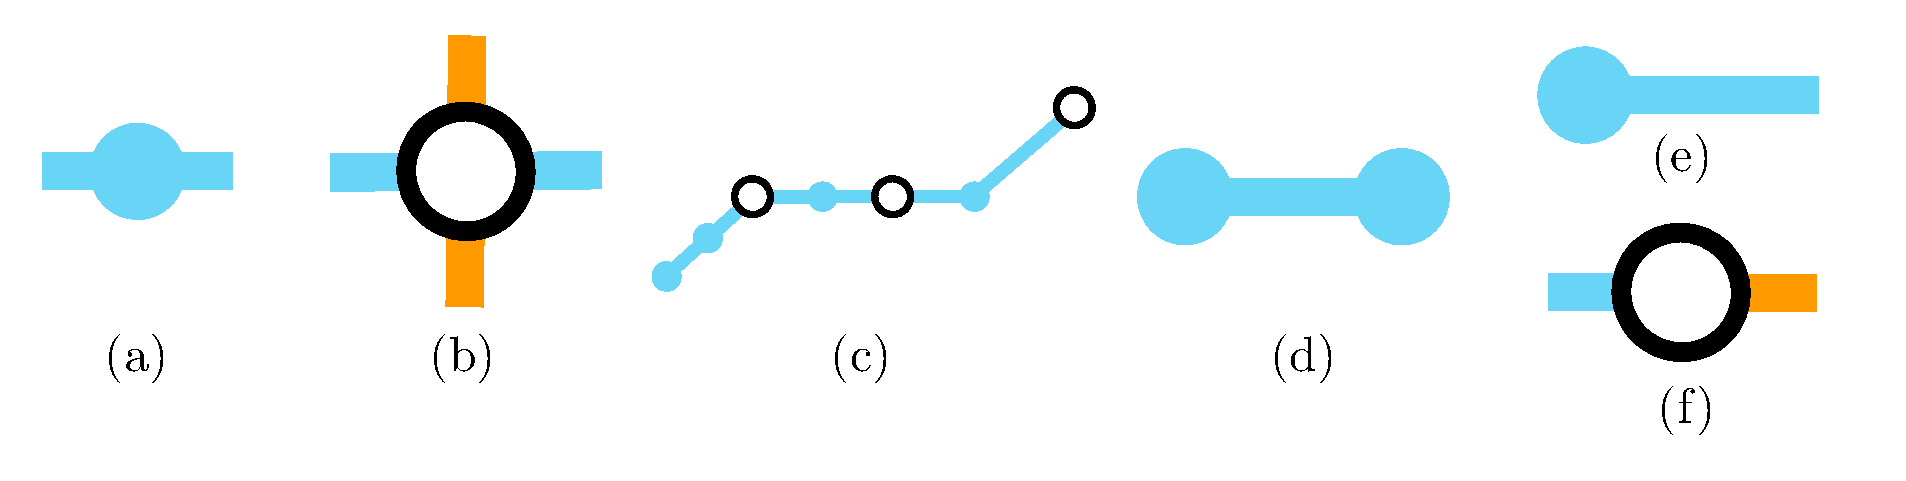
\includegraphics[width=\textwidth]{img/implementation/mapdefinitions.pdf}
	\vspace{-0.5cm}\caption{Left-to-Right: A station (a), an interchange (b), a metro line (c), a link (d), a terminus (e) and a non-terminus station (f).}
	\label{fig:mapdefinitions}
\end{figure}
\begin{description}[leftmargin=7em,style=nextline]
	\item [Station] A single article $v \in V$, represented by a node in the graph. If $v$ has more than two incident edges, i.e an article which spans more than one topic in the graph, it is called an \textit{interchange}.
	\item [Metro Line] A contiguous named path $p \in \Pi$ which is incident to two or more nodes, represented by a line of single colour. Metro lines are composed of \textit{links}.
	\item [Link] A direct edge $e \in E$ between two nodes, which does not pass through any other node. In contrast to \citeauthor{GeneratingInformationMaps}'s definition, here, links must belong to \textit{exactly one} metro line. The case of two lines running side-by-side through the same two nodes is represented by two distinct links. This difference is due only to an implementation detail of the graphing library chosen.
	\item [Terminus] A node with only one incident edge. This is not the definition of a terminus in the sense of the underlying metaphor, since by our definition, a station which is the terminus for two lines (see Figure \ref{fig:mapdefinitions}.f) is no longer categorised as a terminus at all. Instead, the definition requires that the position of a terminus only determine the position of a single link in the graph.
\end{description}

We now turn our attention to transforming the metro map structure into a planar embedding of stations and the metro lines which connect them. As we have previously observed, not all graph layouts were created equal, and the aesthetic quality of a graph-based visualisations has a notable influence on their usability and ease of interpretation \citep{TheBasisForGraphDrawingAlgorithms, WhichAesthetic, AutomaticMetroMapLayoutThesis, AutomaticMetroMapLayout}. 

In \citeauthor{AutomaticMetroMapLayoutThesis}'s words: ``[The] visualisation process is deeply rooted in the human interpretation of the graph as a structure and as such, the quality of the aesthetics of a particular drawing of a graph are very important.'' \citep[p.24]{AutomaticMetroMapLayoutThesis}

We therefore devote a significant amount of thought to optimising the visual quality of the generated metro maps by revisiting \citeauthor{AutomaticMetroMapLayoutThesis}'s aesthetic criteria for layouts, discussed in Chapter \ref{c:litreview}. We justify which of these apply to our visualisations, and for those which are, we detail the methodology used to implement them.

\subsection{\citeauthor{AutomaticMetroMapLayoutThesis}'s Criteria Metro Map layouts}

The set of rules and criteria defined by \cite{AutomaticMetroMapLayoutThesis} form a complex multicriteria optimisation function. Starting with an initial layout, nodes are embedded on a square grid of finite size, and iteratively moved to maximise the node movement criteria, as long as movement does not violate one of the node movement rules.

It should be noted that the function also applies to the positioning of labels and the maximum of a set of label movement criteria alongside the node movement criteria, but as visualisations are unlabelled, these will not be described.

As previously discussed, there are six node movement criteria, which -- using the metro map-specific terms defined above -- are as follows:
\begin{itemize}
	\item\textbf{Angular Resolution}: Maximise the angle of incident links on the same metro line at each station. As \cite{WhichAesthetic} found satisfying this criteria had no statistical effect on task performance, this will not be a priority\footnote{However, as angular resolution comes as a natural consequence of maximising line straightness, it is not disregarded completely during implementation.}.
	
	\item\textbf{Edge Length}: Keep all links approximately the same length. This is a criterion which can be implemented by setting a soft constraint using the graphing library, but it will not be considered beyond this constraint.
	
	\item\textbf{Balanced Edge Length}: Keep links incident to a given station approximately the same length. While it would be possible to implement this as another soft constraint, there is no evidence that it would significantly improve usability, so this will not be considered.
	
	\item\textbf{Edge Crossings}: Minimise the number of link crossings. \citeauthor{WhichAesthetic} found this to be the most significant factor in determining task performance, therefore it will be considered.
	
	\item\textbf{Line Straightness}: Maximise the collinearity of links on the same metro line. \citeauthor{WhichAesthetic} found this criterion to be somewhat beneficial to task performance, so this is both a realistic and justified constraint which will be considered. 
	
	\item\textbf{Octilinearity}: Draw links at multiples of 45$^{\circ}$. Although \citeauthor{WhichAesthetic} found orthogonal graphs to be insignificant factors on task performance, there is a strong argument that the familiarity of the metro map metaphor hinges on certain similarities being preserved. Octilinearity is a noticeable design feature in the metro maps of the world, and therefore should be attempted in our visualisations.
\end{itemize}

We therefore consider minimising edge crossings to be the highest weighted criterion, followed jointly by maximising line straightness and octilinearity.

\subsection{Initial Force-Directed Positioning}

A major difference between the maps generated using this system and maps representing real transit networks is the lack of ``real'' starting positions we have for stations. While the freedom to move points around without having to preserve their relative positioning removes one layout constraint, finding a set of starting positions for the map layout which define a planar embedding with minimal line crossings is non-trivial. 

As \citeauthor{AutomaticMetroMapLayoutThesis} notes, ``This [difficulty] is due to our method being based on optimising an existing layout: if the initial embedding is not adequate, then our method may struggle to produce an acceptable optimisation.''\cite[p.210]{AutomaticMetroMapLayoutThesis}. One solution he suggests is to generate positions using a force-directed algorithm; a class of algorithms which simulate the forces of real physical motion to position nodes in a graph, with minimal edge crossings and approximately uniform edge lengths \citep{springembedders}. The downside to using a force-directed approach is that initial positioning and therefore the final map layout becomes nondeterministic. 

D3.js includes an optimised implementation of \possessivecite{forcedirected} force-directed layout algorithm, and provides several parameters which can be used to alter the forces applied to some or all of the nodes in the graph. The two forces we will adjust to optimise the force-direction for metro maps are as follows:
\begin{itemize}
\item\texttt{force.charge([charge])}\footnote{\url{https://github.com/d3/d3-3.x-api-reference/blob/master/Force-Layout.md\#charge}}\par
	\textit{Charge} specifies the force of attraction between nodes, with negative values causing nodes to repel each other. In order to minimise crossings, this should be a large negative value, particularly for nodes which of higher degrees, which will be surrounded by more edges. We therefore set charge to -500 for nodes with weight $>$ 1, and -300 otherwise. 

\item\texttt{force.alpha([alpha])}\footnote{\url{https://github.com/d3/d3-3.x-api-reference/blob/master/Force-Layout.md\#alpha}}\par
	\textit{Alpha} is the graph's cooling parameter, decaying as the simulation converges on a stable layout. As the temperature falls, node movement slows down, and eventually alpha will drop below a threshold which pauses the simulation, preventing further movement. 
\end{itemize}

Unfortunately, the implementation of \texttt{d3.layout.force} lacks any further mechanism for detecting or reducing line crossings due to the computational expense of the best known algorithms (this subproblem is also NP-Hard). Even if line crossings could be detected, it is likely that the topology of certain graphs generated would make it impossible to find a planar embedding with no crossings.

The parameter \texttt{force.alpha} is re-evaluated every time the simulation is advanced by a single step, which happens approximately 60 times per second. Since our aim is to generate an initial layout with minimal line crossings which will result in the best possible map, we can constantly vary \texttt{force.alpha} based on the quality of the map as its stations are repositioned. Therefore, if the stations settle into a map layout with desirably high octilinearity and good line straightness, the energy of the graph will be reduced such that it is impossible for the embedding to change. Likewise, if the stations start repelling each other in a way that worsens line straightness and octilinearity, the system will have its energy increased and will be more likely to move out of the undesirable state.

The measure of quality that we use to adjust \texttt{force.alpha} is function of the two remaining chosen aesthetic criteria; octilinearity and line straightness. The means by which these two properties are calculated are described in the following sections.

\subsubsection{Octilinearity}

Octilinearity (Equation \ref{eqn:octilinearity} \citep{AutomaticMetroMapLayoutThesis}) penalises lines which are not drawn at multiples of 45$^{\circ}$ angles; the further the gradient of a link in the graph is from a multiple of 45$^{\circ}$, the higher its octilinearity. Lower values are desirable, with zero indicating a graph is entirely octilinear. 

\begin{equation}
	\text{octilinearity}(G) = \sum_{u, v\in E}\bigg|sin\;4\,\bigg(tan^{-1}\frac{|u.y - v.y|}{|u.x - v.x|}\bigg)\bigg|
\label{eqn:octilinearity}
\end{equation}

\begin{figure}[h]
\centering
\begin{minipage}{.4\textwidth}
  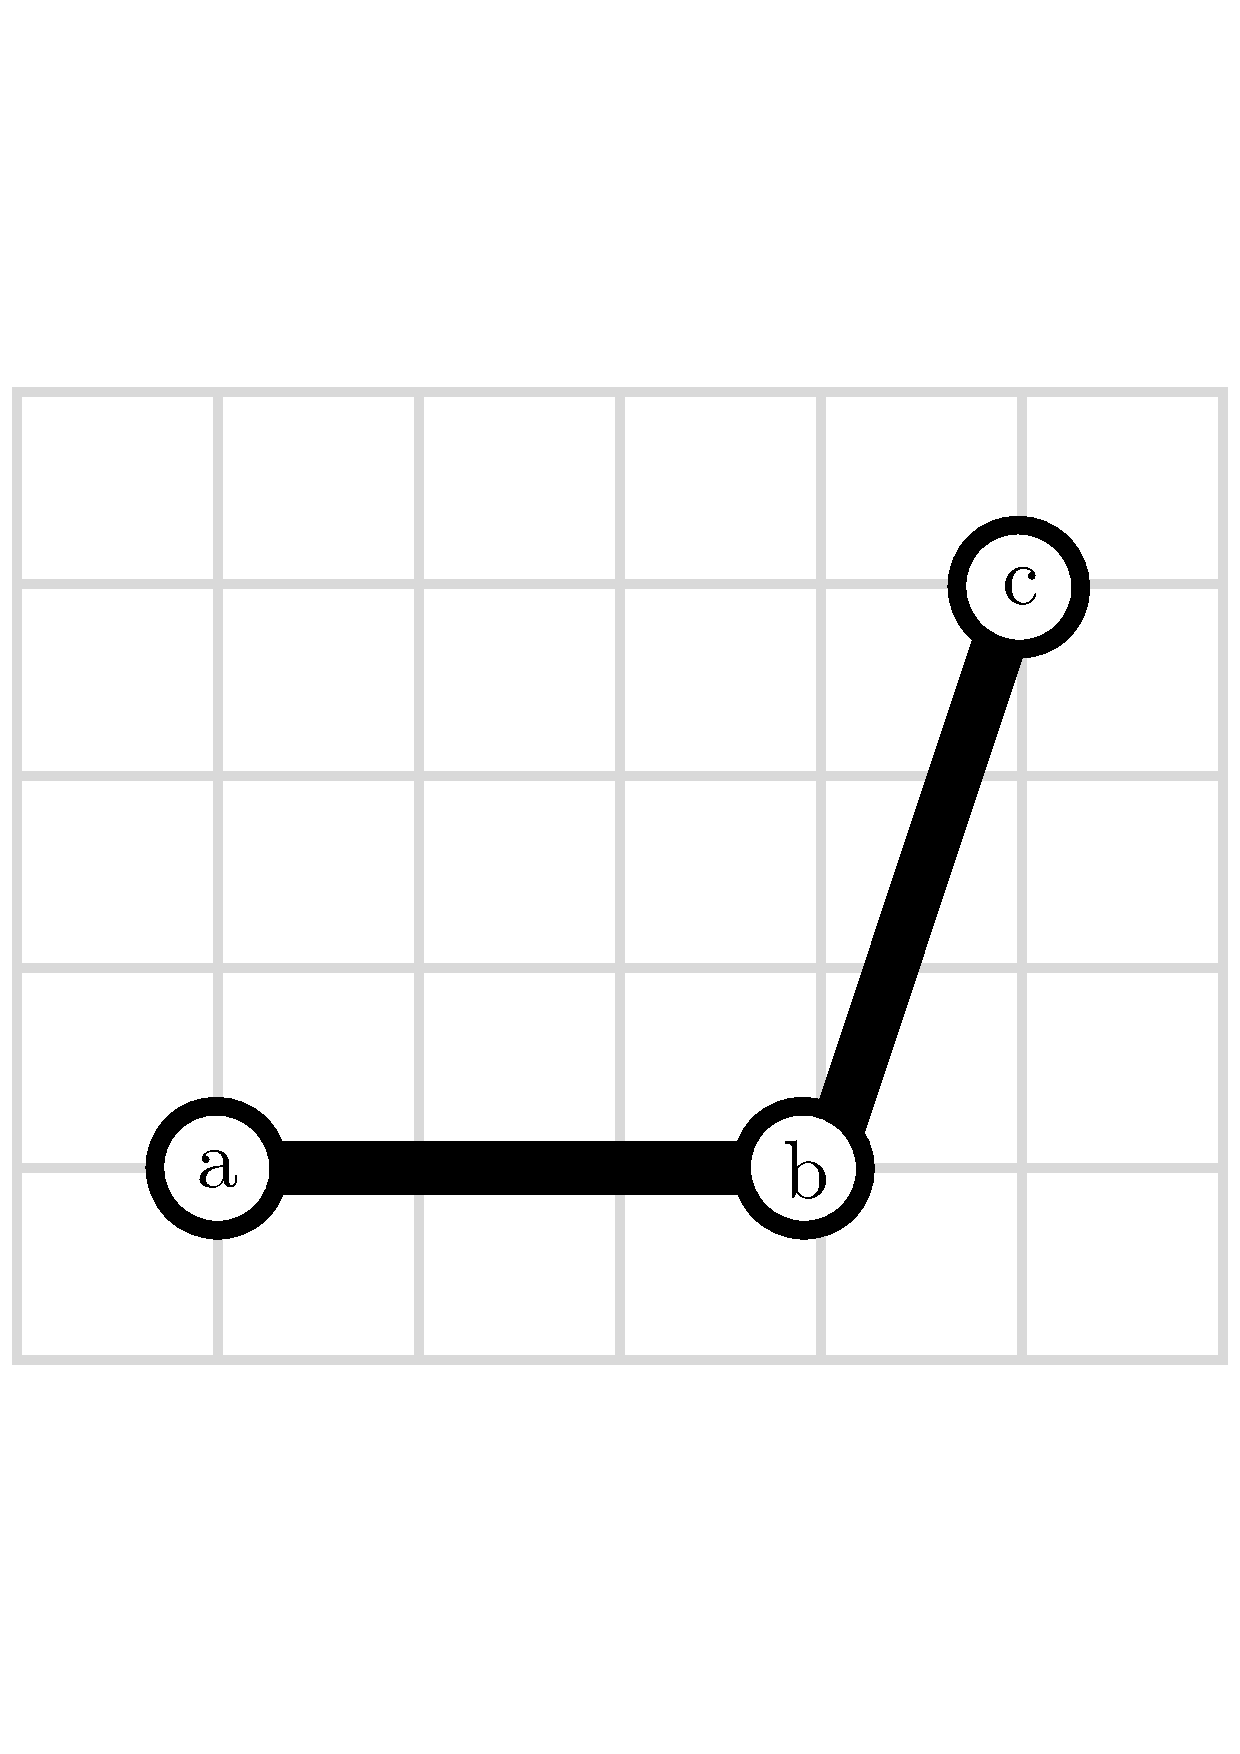
\includegraphics[width=.9\linewidth]{img/implementation/octilinearity.pdf}\caption{Octilinearity Calculation\label{fig:octilinearity}}
  \end{minipage}\hspace{0.5cm}\begin{minipage}{.55\textwidth}
We can calculate the octilinearity of the graph in Figure \ref{fig:octilinearity} (left) as follows, taking positions relative to $(0, 0)$ in the bottom left corner. Algorithm \ref{alg:octilinearity} describes this calculation.
$$\begin{aligned}
\text{octilinearity}(a, b) &= |sin\;4\,(tan^{-1}\frac{|1 - 1|}{|4 - 1|})| = 0 \\
\text{octilinearity}(b, c) &= |sin\;4\,(tan^{-1}\frac{|4 - 1|}{|5 - 4|})| = 0.96 \\[0.1cm]
\text{octilinearity}(a, b, c) &= 0 + 0.96 = 0.96
\end{aligned}$$
\end{minipage}
\end{figure}

There is a caveat to this formula which goes unmentioned by \citeauthor{AutomaticMetroMapLayoutThesis}, but which is necessary to emphasise as a detail of implementation. In the case where $u.x - v.x = 0$, we take octilinearity to be zero, as this value indicates a straight vertical line. Otherwise, attempting to calculate the inverse tangent of a fraction whose denominator is zero (this is mathematically valid, as the principle value of $\tan^{-1}\infty$ is $\frac{\pi}{2}$), which would result in undefined behaviour.\\
\begin{algorithm}
\label{alg:octilinearity}
 \caption{Calculating Map Octilinearity}
 \KwData{$\mathcal{M}$: a metro map $(G=(V, E), \Pi)$}
 \KwResult{$oct \in \mathbb{Q}, 0 \leq oct \leq \frac{24}{25}|E|$: the octilinearity of $\mathcal{M}$}
 $oct \gets 0$ \;
 \ForEach{$e \in E$}{
   $\delta_x \gets |e.source.x - e.target.x|$ \;
   $\delta_y \gets |e.source.y - e.target.y|$ \;
   
   \uIf{$\delta_x = 0 \cup \delta_y = 0$}{
   	 $slope \gets 0$ \tcc*[f]{This avoids a potential division by zero.}}
   	 \Else{
   	  $slope \gets \dfrac{\delta_y}{\delta_x}$ 
    }
   $\theta \gets |sin(4\times{} tan^{-1}(slope))|$ \;
   $oct \gets oct + \theta$ \;
}
\end{algorithm}

\subsubsection{Line Straightness}

The line straightness (Equation \ref{eqn:linestraightness} \citep{AutomaticMetroMapLayoutThesis}) criterion is defined as the sum of every `turn' a metro line makes between its first and last stations, where a turn is measured as the angle between the new link direction and the continuation of the previous direction. The global line straightness is simply the sum of the straightness of every metro line in the map, and as with octilinearity, lower values are preferred.

\begin{equation}
	\text{lineStraigtness}(G) = \sum_{p\,\in{\Pi}}\sum_{u, v\in p} \theta(u, v)
\label{eqn:linestraightness}
\end{equation}

\begin{figure}[h]
\centering
\hspace{-0.5cm}\begin{minipage}{.5\textwidth}
  \centering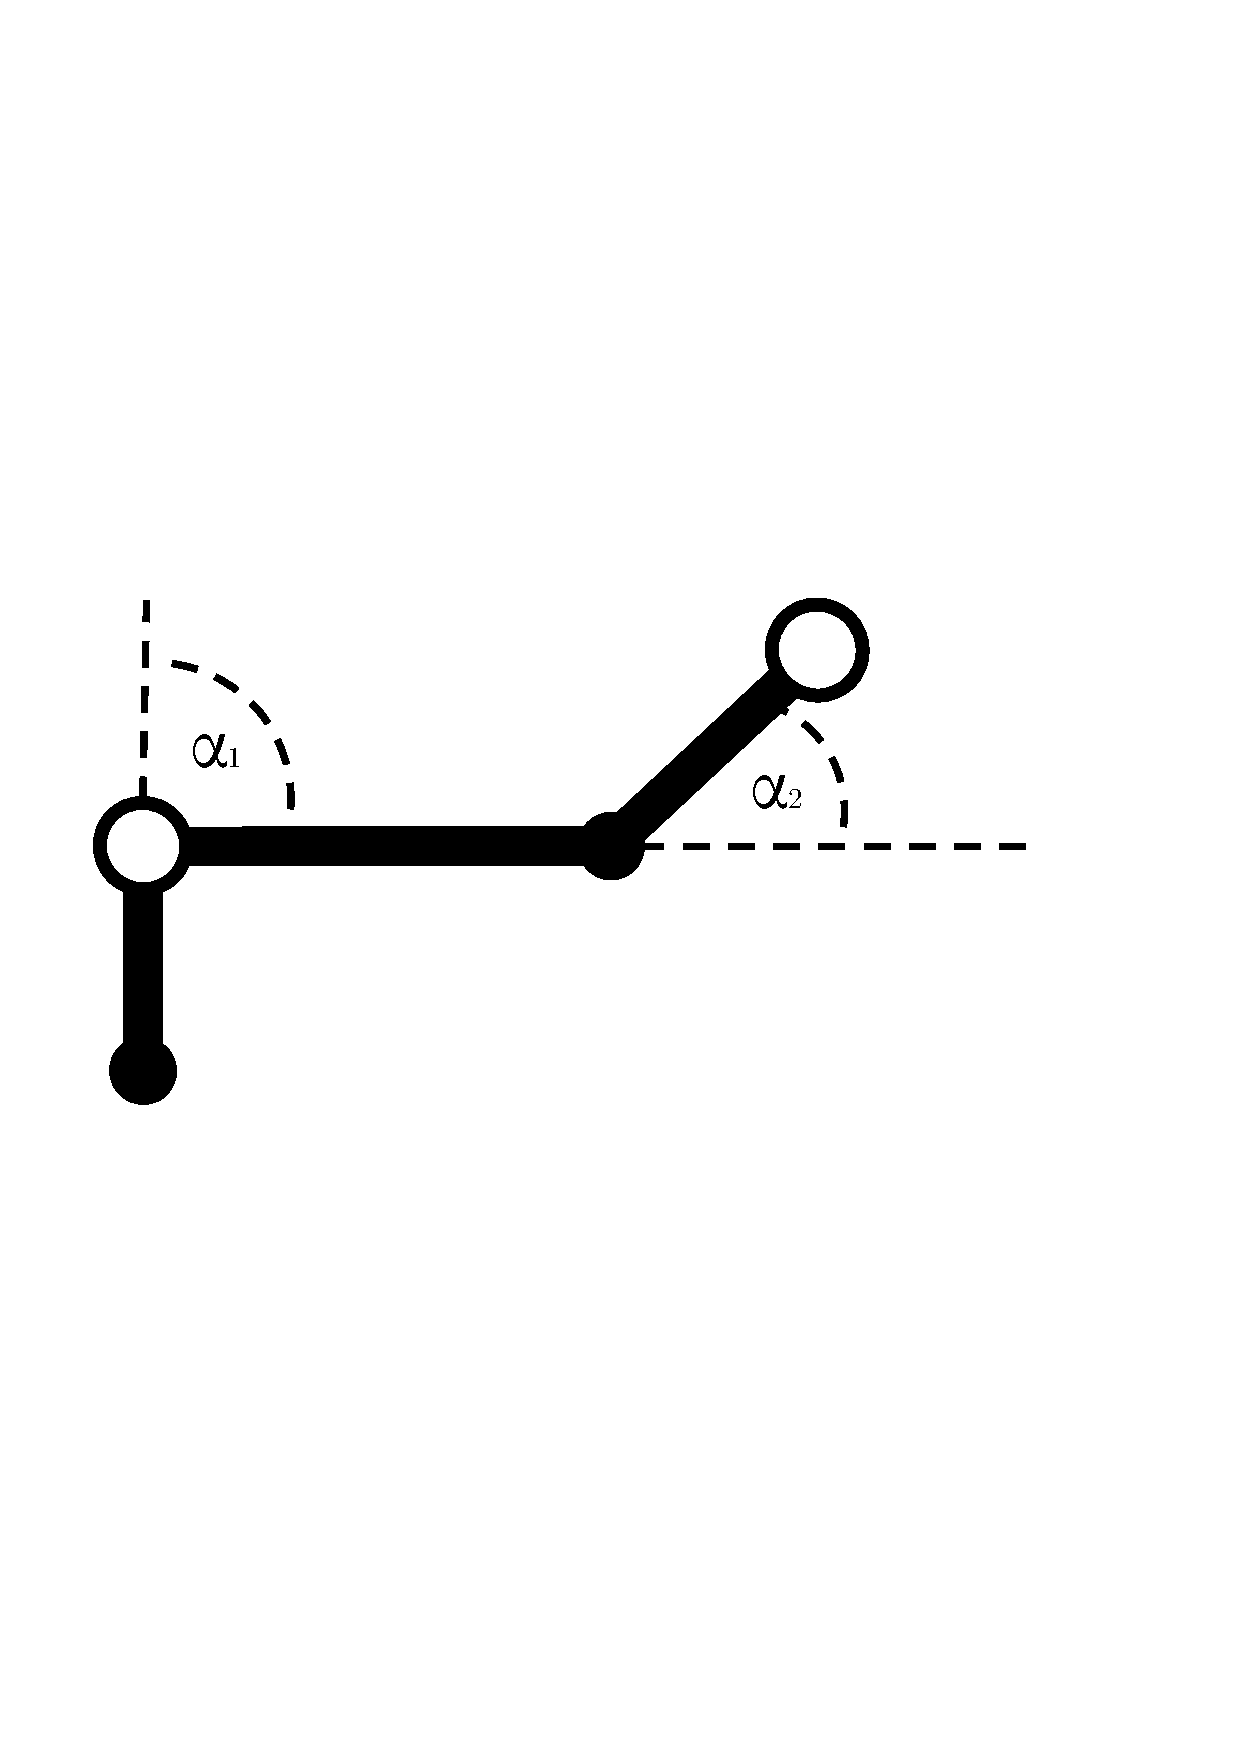
\includegraphics[width=.8\linewidth]{img/implementation/linestraightness.pdf}\caption{Line Straightness Calculation\label{fig:linestraightness}}
  \end{minipage}\hspace{0.5cm}\begin{minipage}{.5\textwidth}
The line straightness of the graph in Figure \ref{fig:linestraightness} (left) is therefore $\alpha_1 + \alpha_2$, where the values of $\alpha_1$ and $\alpha_2$ can be found geometrically from the direction of the links (Algorithm \ref{alg:ls}).
\end{minipage}
\end{figure}

\begin{algorithm}
\label{alg:ls}
 \caption{Calculating Map Line Straightness}
 \KwData{$\mathcal{M}$: a metro map $(G=(V, E), \Pi)$}
 \KwResult{$ls \in \mathbb{Q}, ls > 0$: the line straightness of $\mathcal{M}$}
 $ls \gets 0$ \;
 \ForEach{$p \in \Pi$}{
 	\tcc{Greedily iterate over all 3-tuples of adjacent stations on $p$}
   \ForEach{$(a, b, c) \in p$}{
   \vspace{0.15cm}
   $v_1 \gets \dfrac{\overrightarrow{ab}}{|\overrightarrow{ab}|}$ ; $v_2 \gets \dfrac{\overrightarrow{bc}}{|\overrightarrow{bc}|}$ ;\tcc*[f]{Normalise the two vectors to unit length}
   \vspace{0.15cm}
   $\theta \gets cos^{-1}(v_1.x\times v_2.x + v_1.y\times v_2.y)$ ;\tcc*[f]{Find the angle between links}
   $ls \gets ls + \theta$ \;
   }
}
\end{algorithm}

Empirically, we found the best results came from weighting octilinearity and line straightness equally when using them to set \texttt{force.alpha}, but this could be refined through further investigation. We take the sum of the natural log of both values, to ensure that small improvements to already low values for either criterion are rewarded.

\subsection{Heuristic Refinement}

Once all stations have been assigned their starting positions, we can start incrementally moving them to improve the quality of the map. The first step is to discretise the search space for station positions, by \textit{snapping} stations to intersections on a large grid. We found the optimal size for this grid to be $\frac{n}{4}\times\frac{n}{4}$ for a map containing $n$ stations. 
\begin{figure}[htbp!]
	\centering
	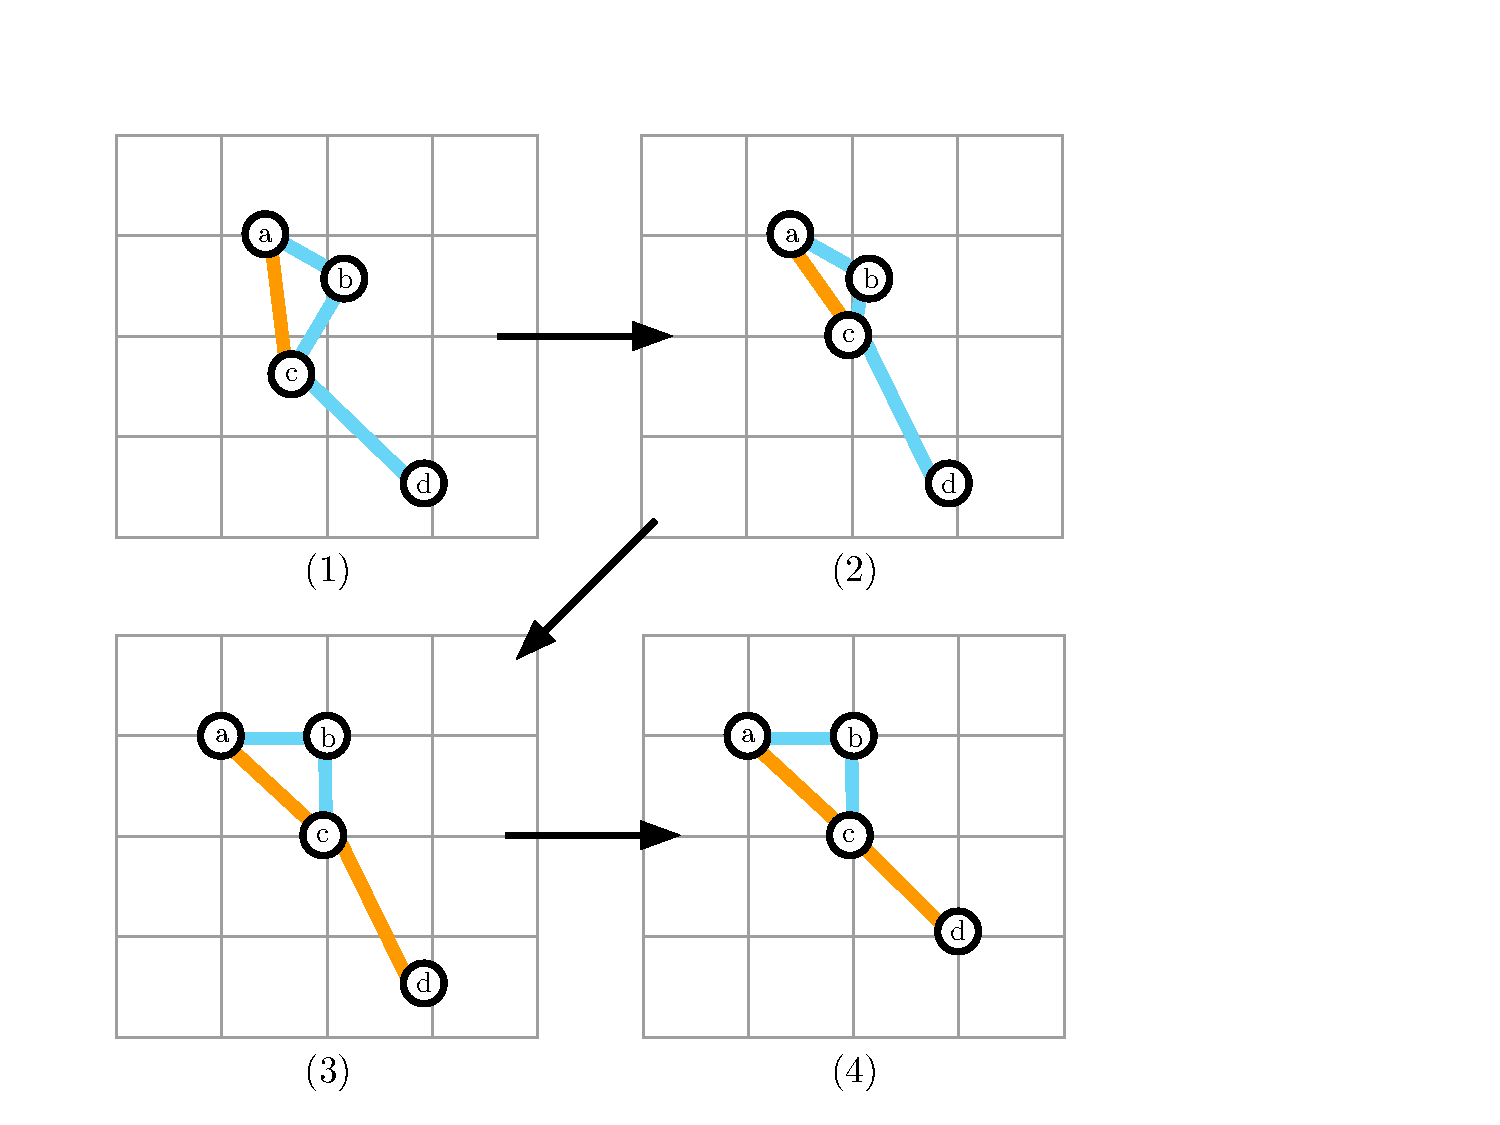
\includegraphics[width=.9\textwidth]{img/implementation/snap.pdf}
	\caption{An example demonstrating the \textit{snap-to-grid} process}
	\label{fig:snap}
\end{figure}

Figure \ref{fig:snap} shows the \textit{snap-to-grid} process applied to a small example. We snap stations in order of descending weight (number of incident edges), as typically the more edges a node is connected to, the more difficult it is to place. In the example, this means station $c$ (with weight three) is moved first. There is contention for the second move, as both stations $a$ and $b$ have weight two, so we make an arbitrary decision as to which we move first, and the two moves are shown as one step. The final station to move is station $d$, after which we can mark all stations as successfully placed. 

Stations whose nearest intersections are already occupied are left unplaced. This implementation contrasts slightly with \citeauthor{AutomaticMetroMapLayoutThesis}'s approach, where stations are snapped \textit{in order} of Euclidian distance to their nearest intersection, and snapped to the next-nearest if the closest intersection is already occupied. We found this implementation performed poorly for maps with several highly connected nodes, which is a common due to news providers often publishing review articles which span many of the lines on the map.

To determine the final station positions, our approach now diverges from \citeauthor{AutomaticMetroMapLayoutThesis}'s into a heuristic method which has been refined for metro maps comprising between 10 and 50 stations. It is vital that metro lines with high affinity have been removed before this stage, or the following process will result in a map where nodes with high weights are occluded.

Although by definition the \textit{snap-to-grid} gives a map near-perfect octilinearity, it can significantly worsen line-straightness, as shown in Figure \ref{fig:aoct}. It would be preferable to have the circled station repositioned as the transformation shows, even though this sacrifices the uniform edge length of the map. We therefore make several passes over each metro line, moving stations to the midpoint of the line between the previous and next neighbouring stations if that line is octilinear.
\begin{figure}[htbp!]
	\centering
	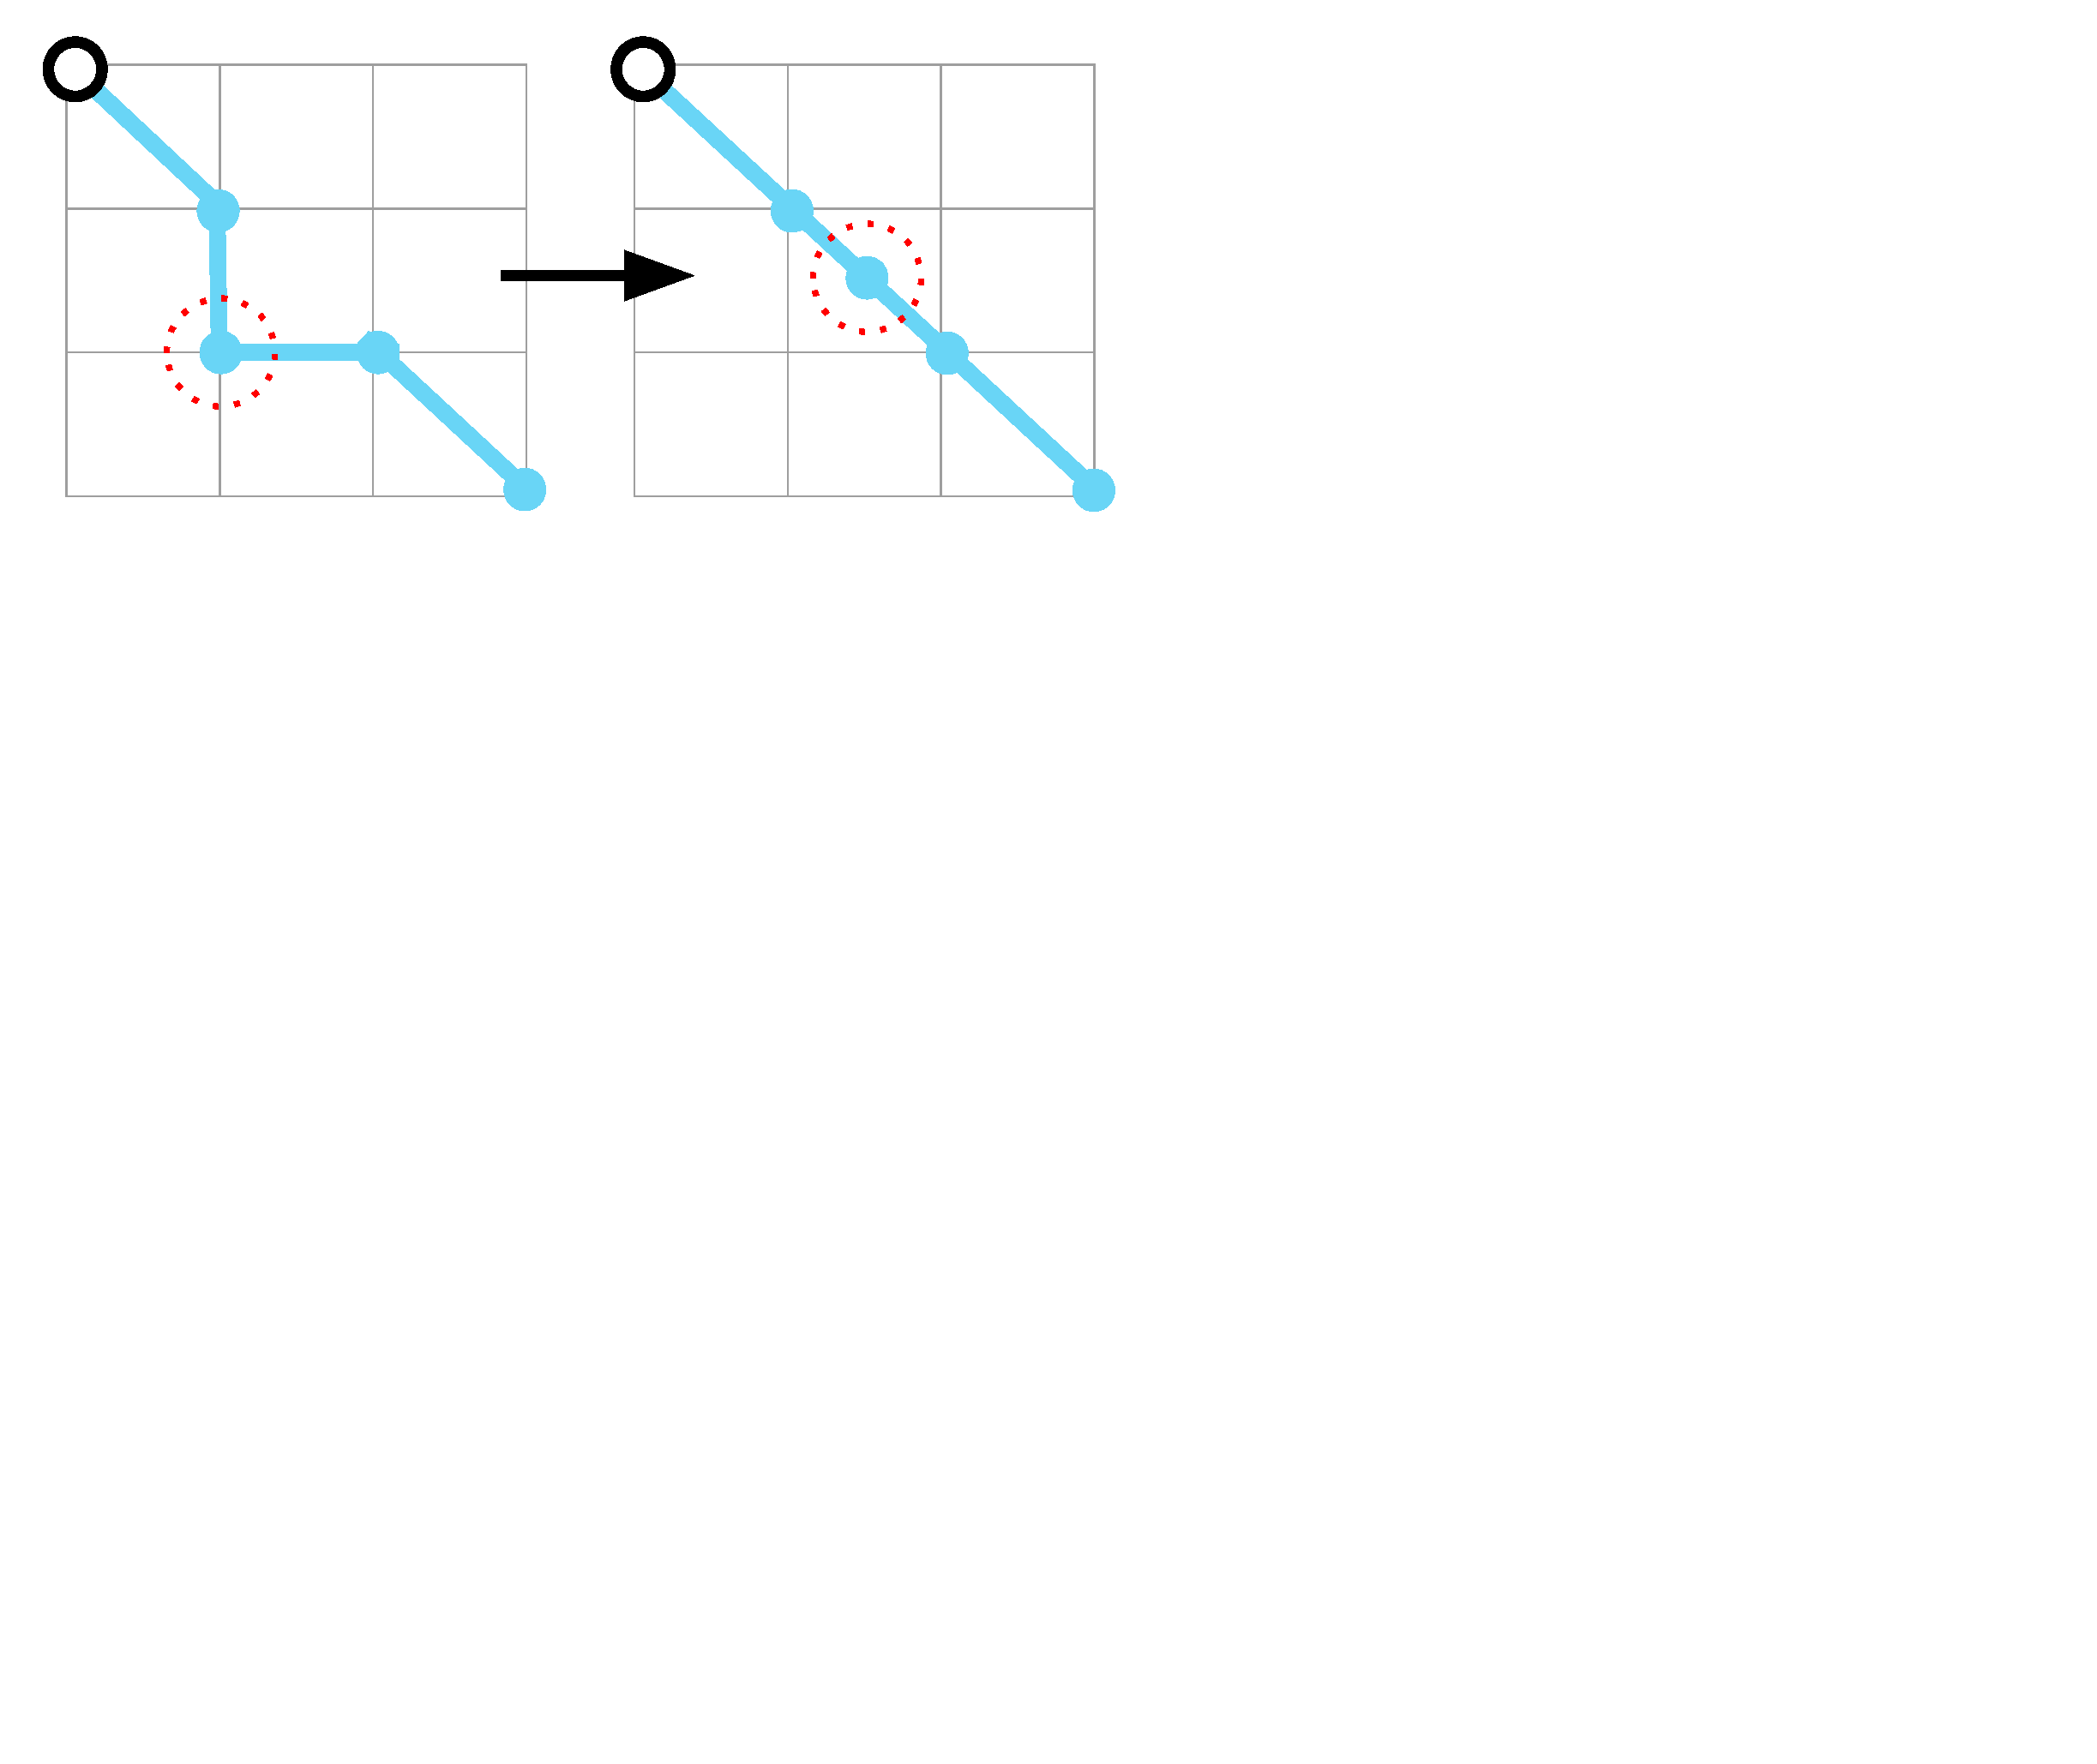
\includegraphics[width=.7\textwidth]{img/implementation/averagingoctilinear.pdf}
	\caption{An octilinear move which compromises the edge-length criterion}
	\label{fig:aoct}
\end{figure}

In addition, a final pass checks for stations which are still unplaced at this point and performs the same midpoint movement regardless of whether the line between the next and previous points is octilinear. This is simply to try and ensure the unplaced point obscures and crosses as few other links as possible in what is most likely a densely packed area of the map. An example of this process is shown in Figure \ref{fig:nonoct}.
\begin{figure}[htbp!]
	\centering
	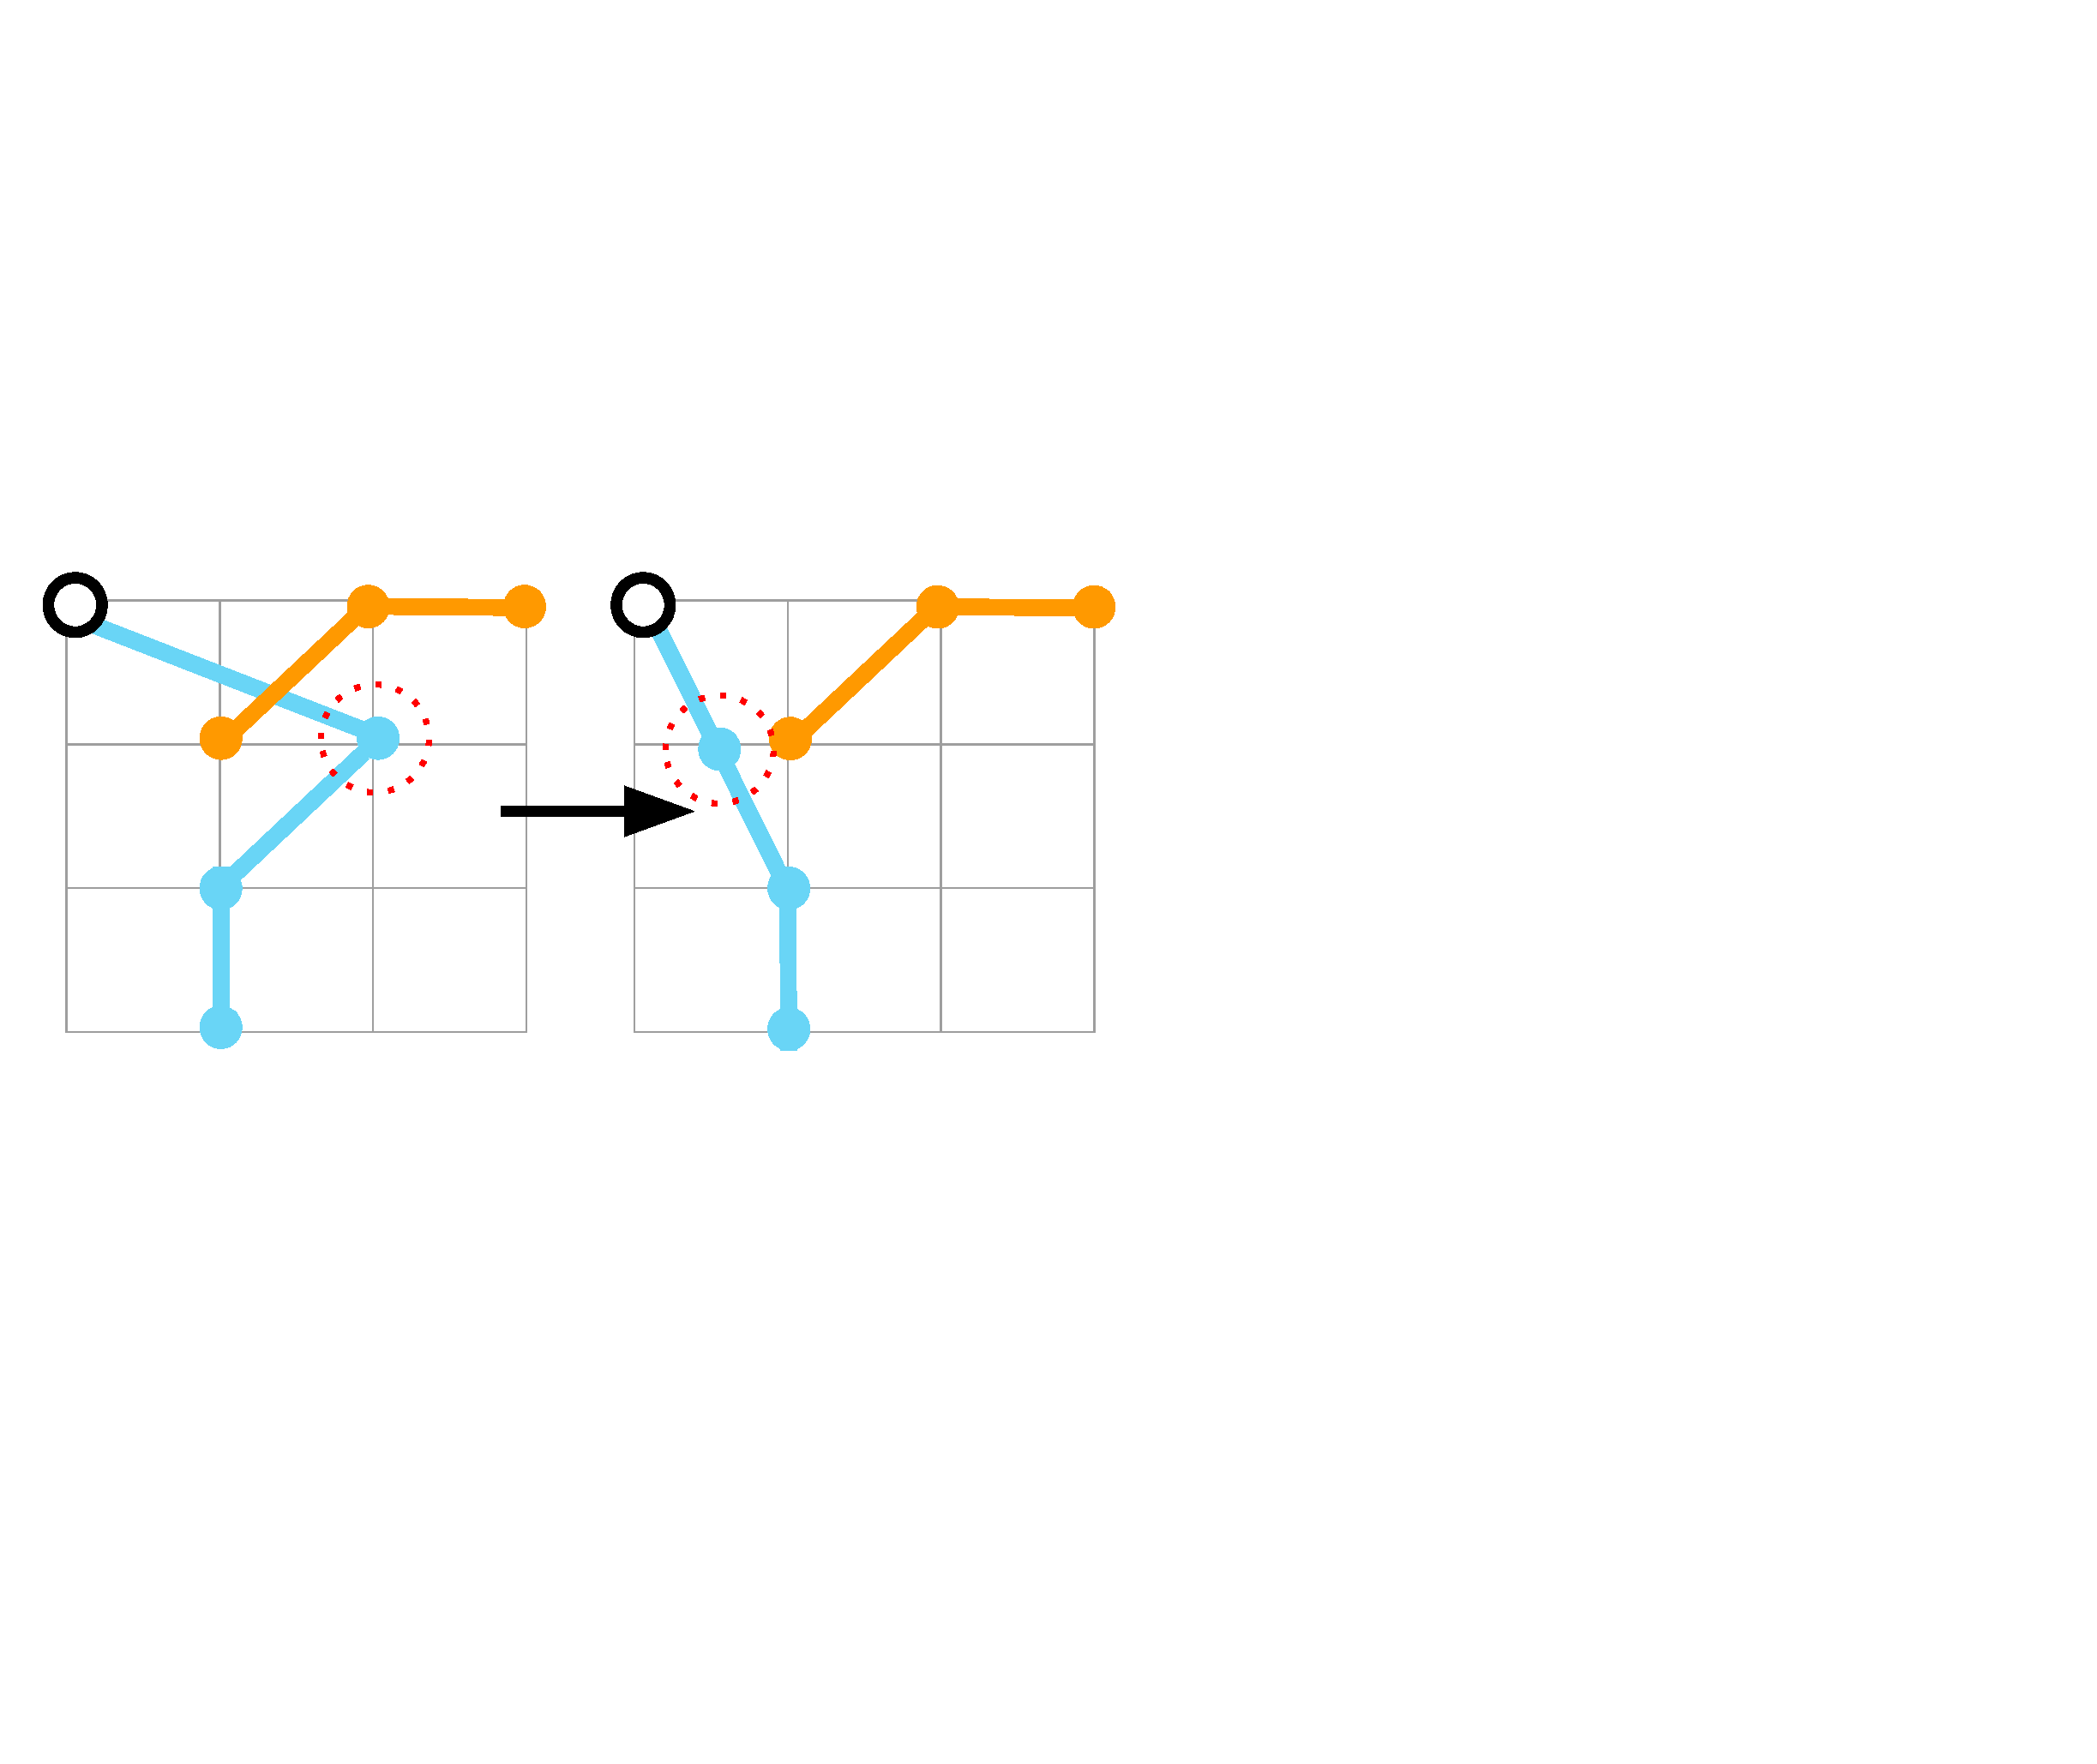
\includegraphics[width=.7\textwidth]{img/implementation/averagingnonoctilinear.pdf}
	\caption{A non-octilinear move of an unplaced station}
	\label{fig:nonoct}
\end{figure}

After the final pass, we recompute octilinearity and line-straightness, and count how many points were left unplaced; i.e. drawn directly on top of another point. If any of the numbers are unsatisfyingly high, the process can be restarted and the randomness of the initial force-direction will result in a different initial embedding.

\section{Summary}

We have given a detailed description of the system's pipeline and the novel transformation of news data from XML elements in an RSS feed to raw text, to parsed keywords, to recognised entities, to nodes in a directed graph, to stations on a formatted metro map.

Several unexpected difficulties arose during implementation, in particularly the tradeoffs involved with entity disambiguation in the context of what makes a ``useful'' metro line, and the process of deciding which lines to select between two or more with high affinity. 

However, the most significant challenge of implementation was undoubtedly the process of drawing usable metro maps. The conflict between edge crossings, line-straightness and octilinearity was omnipresent, and the final algorithm still falls into both local and global minima as it is unable to detect the edge crossings. This section of the pipeline would benefit greatly from further work, as it is a significant area of active research in its own right. As the expected datasets for the map are typically small (under 50 stations),  a non-polynomial time algorithm for refining station positions would be feasible in terms of running time, and would doubtless improve the quality of the maps generated.

The results obtained by using the system to generate metro maps for various news corpora are presented in the next chapter. We take forward the successes of entity disambiguation and denominal adjective stemming, the concepts of line coverage affinity, and the difficulties of generating initial station embeddings as points of discussion.

